%it uses aprilthesis.cls just a simple customisation of the standard book latex package
% with different tips and tricks 
% there is also an extramath.sty package that contains
% macros needed to write physics and mathematics
%
\documentclass[oneside,a4paper,12pt]{aprilthesis}
%
\usepackage[titletoc]{appendix} % appendices
\usepackage[english]{babel}  %good spelling
\usepackage{amssymb,amsmath} %nicer math
\usepackage{fancyhdr}  %funky headers
\usepackage{varwidth} %minipages made easier
\usepackage{makeidx} %index
\usepackage{hepunits}  %gives you units
\usepackage{braket}    %Dirac brakets
\usepackage[hang,small,bf]{caption} %% funky captions
\usepackage[lined,vlined,ruled,linesnumbered]{algorithm2e}  %%% to write pseudocode
\usepackage[backref,colorlinks=true,bookmarks=true,plainpages=false]{hyperref} %links in pdf
\usepackage[sort&compress,numbers]{natbib} %references
\usepackage{hypernat} %references
\usepackage[style=justsymbols,toc,nonumberlist]{glossaries} %glossaries a little bit non standard
%
\makeglossaries
% the file containting the glossary entry
\newglossaryentry{H}% the label
{name={H}, % the term
 description={Hamiltonian}, % brief description
 symbol={\hamiltonian} % the associated symbol
}
\newglossaryentry{H2}% the label
{name={{\hamiltonian}}, % the term
 description={Hamiltonian}, % brief description
 symbol={\hamiltonian$_2$} % the associated symbol
}

\makeindex
%
\title{Time Dependent Tight Binding+U: Applications to Fluorescent Molecules}
\author{Alin Marin Elena}
\acadtitle{Licentiate in Physics}
\affiliation{The Queen's University of Belfast}
\tdesc{A thesis  submitted to the School of Mathematics and Physics\\in partial fulfilment 
of the requirements for the degree of\\Doctor of Philosophy}
%not official asked but nice to have it
\logo[3cm]{figures/qub}
% uncomment if you want a certain date
%\date{April 1, 2008}
%
\hypersetup{%
pdftitle = {Time Dependent Tight Binding+U: Applications to Fluorescent Molecules},
pdfsubject = {Alin M Elena's PhD thesis},
pdfkeywords = {time dependent, tight binding, fluorescent, electronic structure, atoms, molecules, dft, oprimisation},
pdfauthor = {\textcopyright\ Alin Marin Elena}
}
%
\begin{document}
% you get no style for the frontmatter
\pagestyle{empty}
\frontmatter
% generates the title page
% according to QUB requirements
\maketitle
%
%if uncommented will insert a dedication page
%the dedication gets centered in the middle of the page
%first argument is intended to be used only for a short word
%second argument contains the dedication text you can use \\ to break the line 
\makededication{to}{be added}
%
%if uncommented will insert main quote page
% the quote will be centered on the page
% there is another command \chapterquote{}{} that will insert a quote
% aligned to right.
\mainquote{to be decided
}{\quad \quad ....}
%
\chapter{Abstract}
\par{
the last thing that will be added
}
%
\chapter{Acknowledgement}
\par{
wil be added later
}

%
\setcounter{tocdepth}{1}
\tableofcontents
%
\glsaddall
\renewcommand{\glossaryname}{Glossary of Symbols}
\printglossaries
% the mainmatter is fancy
\mainmatter
\pagestyle{fancy}
% it is simple to include the files
%chapter by chapter
% the introduction does not get numbered.
% check introduction.tex to see how
\cleardoublepage
\phantomsection
\addcontentsline{toc}{chapter}{Introduction}
\chapter*{Introduction}
\chapterquote{``If a question can be put at all, \\ then it \emph{can} also be answered.''
}{Ludwig Wittgenstein}


\chapterquote{"...if the universities will not study useless subjects, who will?"}{G. F. Fitzgerald, Nature, 45/46, 392 (1892)}

The introductory chapter set goes here.

\chapter[TDTB+UJ]%
{Time Dependent Tight Binding+UJ}
\label{ch:one}
%
 \chapterquote{Le savant n'\'etudie pas la nature parce que cela est utile; \\
\indent il l'\'etudie parce qu'il y prend plaisir, \\
\indent et il y prend plaisir parce qu'elle est belle.}%
{by Henri Poincar\'e}
%
\section{Introduction}
\par{Tight binding is an approach to the quantum mechanical many particle problem particularly valuable in cases
where exact analytic solutions are not available (i.e. almost always) and other numerical approaches
like CI, DFT or GW are too time-consuming.}
\par{Tight binding methods lie between the very accurate and very expensive,
\emph{ab initio} methods, and the fast but limited, empirical methods. The
speed of the tight binding methods compared with the \emph{ab initio} is two
or three order of magnitude faster. Gaining speed we loose from the
transferability of the model, but in tight binding we retain the quantum
nature of the bonding. The tight binding methods are the ideal candidates, at
this time, for large size atomistic simulation in the field of nanostructure materials, molecular devices and biomolecules. Due to the nature of the approximations many flavours of tight binding were developed lately. Some examples: the NRL-TB total energy method\citep{Mehl96}, the density functional TB (DFTB) method \citep{Frauenheim00,Elstner98,Elstner07,Seifert07}, the ab initio TB method (AITB) \citep{Sankey89, Horsfield97, Tu06}, the nonconventional TB method \citep{Khakimov05}, the environment dependent TB method \citep{Tang96}, the orthogonal and nonorthogonal TB method of Voityuk \citep{Voityuk06,Voityuk06b} and extended H\"{u}ckel TB\citep{Rincon08} to cite only few. For an overview see e.g. \citep{Finnis03,Goringe97b}.}
\par{The relation between tight binding and density functional theory was
  investigated by Sutton, Foulkes and Frauenheim in \citep{Sutton88,Foulkes89,Frauenheim00}. In short, they
  prove that DFT can be ''downgraded'' to a tight binding model (DFTB).}
\par{Different approximations made to full DFT total energy functional give us
different tight binding models. A common feature of all tight binding models
is the minimum basis set, that is taking into account  one $s$ orbital,
$3p$-orbitals, $5d$-orbitals
$\{\ket{s},\ket{p_x},\ket{p_y},\ket{p_x},\ket{d_{xy}},\ket{d_{yz}},\ket{d_{zx}},$
$\ket{d_{x^2-y^2}},\ket{d_{3z^2-r^2}}\}$
per atom. Principal quantum numbers do not have any meaning. The main
approximations that would define a tight binding model. Finnis in \citep{Finnis03} gives a list of common  approximations in tight binding} 
\begin{itemize}
  \item{ignoring three centre integrals}
  \item{parametrise two centre integrals}
  \item{ignore non-spherical terms on an atom}
  \item{ignore inter-site Coulomb interactions}
  \item{ignore charge transfers}
  \item{assume orthogonality of orbitals}
  \item{make a real space representation as multi-ion potentials}
  \item{make a real space second moment approximation}
\end{itemize}
\par{Finnis \citep{Finnis03} defines the quality of a tight binding model as the ratio of the predictive power of the model over complexity}
\begin{equation*}
 Q=\textrm{predictive power}/complexity
\end{equation*}
\par{Predictive power is in fact an abuse of concept since we refer to quantities which were already measured or computed via more accurate methods. Finnis \citep{Finnis03} calls it \emph{prediction of the past}. Predictive power is in fact a measure of the \emph{transferability} and tells you how well is computed a quantity which was not involved in the parametrisation process.}
\par{The remainder of this chapter will present the approximations used in our tight binding model.}
\section{From Density Functional Theory to Tight Binding}
\section{scrap}
\par{Usually\marginpar{this should be rewritten and moved somewhere else} a general tight binding model starts with the assumption that the
total energy can be written as}
\be
E=\sum_{i=1}^{N}\epsilon_i+\frac{1}{2}\sum_{i,j,i\neq j}U(R_{ij})
\ee
where $\epsilon_i$'s are the eigenvalues of a Schr{\"o}dinger-like equation
\be
\label{eigenschro}
H\ket{\psi_i}=\epsilon_i\ket{\psi_i}
\ee
$U(R_{ij})$ with $R_{ij}=|\vec{R_j}-\vec{R_i}|$ is a short-range pairwise
potential between the atoms $i$ and $j$.
\par{Eq. \gref{eigenschro} is solved in a minimal basis set of atomic like
localised functions $\{\phi_i\}$ which leads to the well known secular equation}
\be
|\underline{H}-\epsilon \underline{S}|=0
\ee
with matrices $\underline{H}$ and {\underline{S}} defined by
\be
H_{ij}=\bra{\phi_i}H\ket{\phi_j}\quad\quad S_{ij}=\Braket{\phi_i|\phi_j}
\ee
\par{Commonly we call $H_{ij}$ hopping integrals and $S_{ij}$ overlap
integrals. Another common feature is to consider $H_{ij}$, extending only to
first or second neighbours, as parameters taken from experiment or other
calculations. $\underline{S}=\underline{I}$ gives us what we call orthogonal
models.}
\par{Another important step is the use of two centre parametrisation of
Slater-Koster which gives us a fixed number of fundamental hopping integrals
(at least 4 for $sp$-systems - originally denoted as $ss\sigma$, $sp\sigma$,
$pp\sigma$, $pp\pi$). These parameters are interatomic
distances dependent. There is no absolute parametrisation for the interatomic distance
dependence, an exponential or an inverse power law being often used.}
\par{Our aim is to create a time dependent tight binding model which would help us to study
photoelectron transfer (PET) in sensor molecules \citep{deSilva01b}.}
\section[GSP scheme]{Goodwin-Skinner-Pettifor based scheme}
\par{Goodwin-Skinner-Pettifor (GSP) scheme was suggested in \citep{Goodwin89} and improved by Xu \emph{et al.}\citep{Xu92}. A recent improvement is added by Pettifor
\citep{Mrovec04}. The model that we use is based on Xu's implementation of
GSP scheme with two major differences which will be pointed when they would
appear. The total energy is given by}
\be
E=2\text{Tr}[\rho H]+\sum_{i}F\biggl(\sum_{j,i\neq j}\phi(R_{ij})\biggr)-2T_ek_B(\text{Tr}\rho\ln{\rho}+\text{Tr}(1-\rho)\ln{(1-\rho)})
\ee
where $i$, $j$ represents the atoms, $F(x)$ the embedded function for the
repulsive energy, $\phi(R_{ij})$ is the pair repulsive term between atom $i$
and $j$. Last term gives the ``temperature'' dependence of the model. In fact
is a trick used in order to improve the SCF models and to improve molecular dynamics. It represents the product $T_eS$ where
$T_e$ is ``the electronic temperature'' and $S$ is the entropy of a fermionic
gas. This is one of the improvements to the model.
\be
F(x)=\sum_{i=1}^{4}A_ix^i
\ee
with $A_i$'s parameters taken from \citep{Xu92}.
\be
\label{GSPscale}
\begin{split}
h_{\alpha}(r)=&V_{\alpha}\biggl(\frac{r_0}{r}\biggr)^n\exp{\biggl\{n\biggl[-\biggl(\frac{r}{r_c}\biggr)^{n_c}+\biggl(\frac{r_0}{r_c}\biggr)^{n_c}\biggr]\biggr\}}\\
\phi(r)=&\phi_0\biggl(\frac{d_0}{r}\biggr)^m\exp{\biggl\{m\biggl[-\biggl(\frac{r}{d_c}\biggr)^{m_c}+\biggl(\frac{d_0}{d_c}\biggr)^{m_c}\biggr]\biggr\}}
\end{split}
\ee
with $\alpha=ss\sigma,sp\sigma, ...$. $V_{\alpha}$ represents fundamental
hopping integral and $h_{\alpha}$ times angular factor given by Slater-Koster
parametrisation gives the inter site elements of the Hamiltonian. $r_0$
represents the first neighbour distance (bond length at equilibrium in our
case) all the rest quantities from \gref{GSPscale} are parameters to be
fit. $r_c$ is taken to lie somewhere in between first and second neighbours.
\par{Another set of parameters is represented by on-site energies
$\epsilon_{\alpha}$ ($\alpha=s,p,d, ...$)}
\be
\epsilon_{\alpha}^{i}=\bra{\alpha^i}H\ket{\alpha^i}
\ee
\par{To ensure energy conservation to $h_{\alpha}$ and $\phi$ tails are added. They
join the function at $r_1$ and are zero at $r_{cut}$. A simple polynomial form
is implemented such as to have continuous function and derivatives (first and
second) at $r_1$ and a zero function and derivatives (first and second) at
$r_{cut}$. This is the second difference from Xu's model. The tail function is}
\be
t(r)=(r-r_{cut})^3(10c+5br+3ar^2+5br_{cut}+4arr_{cut}+3ar_{cut}^2)/60
\ee
where $a,b,c$ are determined by the restrictions from definition of the
tail. Theirs values are
\be
\begin{split}
a=&\frac{10}{(r_1-r_{cut})^5}(12A-6Br_1+Cr_1^2+6Br_{cut}-2Cr_1r_{cut}+Cr_{cut}^2)\\
b=&-\frac{4}{(r_1-r_{cut})^5}(45Ar_1-21Br_1^2+3Cr_1^3+15Ar_{cut}+12Br_1r_{cut}-4Cr_1^2r_{cut}+9Br_{cut}^2\\&-Cr_1r_{cut}^2+2Cr_{cut}^3)\\
c=&-\frac{1}{(r_1-r_{cut})^5}(-60Ar_1^2+24Br_1^3-3Cr_1^4-60Ar_1r_{cut}+12Br_1^2r_{cut}-36Br_1r_{cut}^2\\&+8Cr_1^2r_{cut}^2-4Cr_1r_{cut}^3-Cr_{cut}^4)
\end{split}
\ee
with $A=f(r_1)$, $B=f^{\prime}(r_1)$, $C=f^{\prime\prime}(r_1)$
\par{This model was implemented in TDTB+UJ and used in all the
calculation presented in this thesis. Figures \gref{ssg} and \gref{spg}
show the radial part of hopping integrals $ss\sigma$ and $sp\sigma$ with a
tail added at $ r_1=1.5 \angstrom $ and a cut-off $ r_{cut}=1.9 \angstrom $, the rest of
parameters are taken from Table \gref{tablenh3} first SSA column and represent
fitted parameters for $N-H$ bond in our GSP-like model.}
\begin{figure}[!htb]
\begin{center}
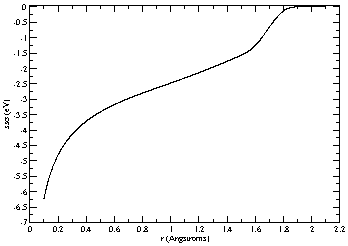
\includegraphics[width=0.75\textwidth]{figures/ssg}
\end{center}
\caption{$ss\sigma$ radial dependence}
\label{ssg}
\end{figure}
%
\begin{figure}[!htb]
\begin{center}
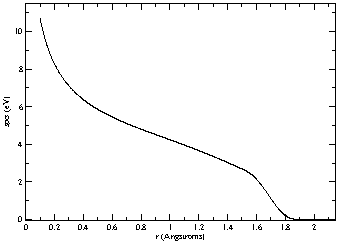
\includegraphics[width=0.75\textwidth]{figures/spg}
\end{center}
\caption{$sp\sigma$ radial dependence}
\label{spg}
\end{figure}
%
\section{Introduction}
\par{The hamiltonian in second quantisation including electron-electron interaction term}
\begin{equation}
H=\sum_{i,\sigma}\epsilon_ia_{i\sigma}^{\dag}a_{i\sigma}+\sum_{i\neq j,\sigma}t_{ij}a_{i\sigma}^{\dag}a_{j\sigma}+\frac{1}{2}\sum_{ijkl\sigma \sigma{\prime}}
V_{ijkl}a_{i\sigma}^{\dag}a_{j\sigma\prime}^{\dag}a_{k\sigma\prime}a_{l\sigma}
\end{equation}
\par{$\sigma$ index stays for spin}
\par{first two terms are "normal" tight-binding terms}
\par{last term is the electron-electron interaction term.}
\par{Expanding the field operators in single particle eigenfunction we get}
\begin{equation}
\begin{split}
V_{ijkl}&=\int\phi_{i}^{*}(\bm{r})\phi_{l}(\bm{r})W(rr\prime)\phi_{j}^{*}(\bm{r^\prime})\phi_{k}(\bm{r^\prime})\td\bm{r}\td\bm{r^\prime}\\
&=\bra{ij}W\ket{lk}
\end{split}
\end{equation}
where $W(rr^\prime)=\frac{1}{4\pi\epsilon_0}\frac{e^2}{|\bm{r}-\bm{r^\prime}|}$.
\par{Electron-electron interaction from the point of view of field theory is: two particles in states $(l\sigma,k\sigma^\prime)$ interact and as a result two particles
in the states $(i\sigma,j\sigma^\prime)$ emerge. Because of the nature of the hamiltonian, non-relativistic, the spin is conserved (no spin flip is described).}
\par{In tight-binding usually we ignore all the interactions described by such schemes.}
\par{Two type of such integrals are important for us direct and exchange Coulomb integrals.}
direct Coulomb integrals
\begin{equation}
\label{udef}
V_{ijji}=\int\phi_{i}^{*}(\bm{r})\phi_{i}(\bm{r})W(rr\prime)\phi_{j}^{*}(\bm{r^\prime})\phi_{j}(\bm{r^\prime})\td\bm{r}\td\bm{r^\prime}=U_{ij}
\end{equation}
$U_{ii}$ is the interaction energy associated with putting an elctron of spin up, let's say, into an orbital where there is already an electron with spin down.\\
exchange Coulomb integrals
\begin{equation}
V_{ijij}=\int\phi_{i}^{*}(\bm{r})\phi_{j}(\bm{r})W(rr\prime)\phi_{j}^{*}(\bm{r^\prime})\phi_{i}(\bm{r^\prime})\td\bm{r}\td\bm{r^\prime}=J_{ij}
\end{equation}
exchange energy only affects like spin electrons.
\par{Using the definition of $U$ from \gref{udef} we get a value of order $20eV$ which
disagrees with experimental results. This come from the fact that the basis set is incomplete.
The incompletness of the basis set exclude any virtual transitions to these states.}
\par{+U formalism describes correctly the discontinuity in the potential as the occputaion number is changed (???Janak's theorem???).}
\section{The model}
\par{Assumptions:}
\begin{itemize}
\item{Not all electrons are correlated. These are separated out from the others identified by the orbitals they occupy or region of space or both.}
\item{When replacing an expectation value it is assumed that correlation exists only between electrons whose orbitals are on the same atom. }
\item{Only electrons with the same $n$within an atom are correlated}
\item {We use the \textit{mean field approximation} -- the two electron operator is expressed in term of a one electron operator acting alone but in the average field of the other}
\end{itemize}
\par{So, the expectation value of electron-electron interaction operator becomes}
\begin{equation}
\begin{split}
\frac{1}{2}&\sum_{ijkl\sigma\sigma^\prime}V_{ijkl}\langle a_{i\sigma}^{\dag}a_{j\sigma^\prime}^{\dag}a_{k\sigma^\prime}a_{l\sigma}\rangle
\cong \frac{1}{2}\sum_{ijkl\sigma\sigma^\prime}V_{ijkl}(\langle a_{i\sigma}^{\dag}a_{l\sigma} \rangle \langle a_{j\sigma^\prime}^{\dag}a_{k\sigma^\prime} \rangle -
\langle a_{i\sigma}^{\dag}a_{k\sigma^\prime}\rangle \langle a_{j\sigma^\prime}^{\dag}a_{l\sigma} \rangle )\\
&=\frac{1}{2}\sum_{ijkl\sigma\sigma^\prime}V_{ijkl}(n_{il}^{\sigma\sigma}n_{jk}^{\sigma^\prime\sigma^\prime}-
n_{ik}^{\sigma\sigma^\prime}n_{jl}^{\sigma^\prime\sigma})
\end{split}
\end{equation}
\par{$n_{ij}^{\sigma\sigma^\prime}$ = generalised occupation numbers. (density matrix with non zero off-diagonal elements)}
\par{Each index $ijkl$ stands for a $ \lbrace \bm{R}nlm \rbrace $ set, but having in mind our assumptions we realise
that $l,m$ are the only one which differs. We replace ${ijkl} \rightarrow {L_1L_2L_3L_4}$ with $L_i \rightarrow \lbrace l_im_i \rbrace$ and we get}
rewrite from here
\begin{equation*}
\begin{split}
E^U&=\frac{1}{2}\sum_{\{m_i\}\sigma\sigma^\prime}V_{m_1m_2m_3m_4}
(n_{m_1m_4}^{\sigma\sigma}n_{m_2m_3}^{\sigma^\prime\sigma^\prime}-
n_{m_1m_3}^{\sigma\sigma^\prime}n_{m_2m_4}^{\sigma^\prime\sigma})\\
&=\frac{1}{2}\sum_{\{m_i\}\sigma\sigma^\prime}V_{m_1m_2m_3m_4}
n_{m_1m_4}^{\sigma}n_{m_2m_3}^{\sigma^\prime}-\frac{1}{2}\sum_{\{m_i\}\sigma}V_{m_1m_2m_3m_4}
n_{m_1m_3}^{\sigma}n_{m_2m_4}^{\sigma}\\
&=\frac{1}{2}\sum_{\{m_i\}\sigma}V_{m_1m_2m_3m_4}n_{m_1m_4}^{\sigma}n_{m_2m_3}^{-\sigma}\\&-
\frac{1}{2}\sum_{\{m_i\}\sigma}V_{m_1m_2m_3m_4}
(n_{m_1m_3}^{\sigma}n_{m_2m_4}^{\sigma}-n_{m_1m_4}^{\sigma}n_{m_2m_3}^{\sigma})
\end{split}
\end{equation*}
\begin{equation}
\label{Eu}
\begin{split}
E^U=&\frac{1}{2}\sum_{\{m_i\}\sigma}V_{m_1m_2m_3m_4}n_{m_1m_4}^{\sigma}n_{m_2m_3}^{-\sigma}\\+&
\frac{1}{2}\sum_{\{m_i\}\sigma}(V_{m_1m_2m_3m_4}-V_{m_1m_2m_4m_3})
n_{m_1m_4}^{\sigma}n_{m_2m_3}^{\sigma}
\end{split}
\end{equation}
%
\par{The interaction potential associated with $E^U$ is given by}
\begin{equation*}
\p{E^U}{n_{mm^\prime}^{\sigma^\prime}}
\end{equation*}
%
\par{For simplicity we will compute it in two steps}
%
\begin{equation}
\begin{split}
V^{(1)}&=\frac{1}{2}\p{}{n_{mm^\prime}^{\sigma^\prime}}\sum_{\{m_i\}\sigma}V_{m_1m_2m_3m_4}n_{m_1m_4}^{\sigma}n_{m_2m_3}^{-\sigma}\\
&=\frac{1}{2}\sum_{\{m_i\}\sigma}V_{m_1m_2m_3m_4}(n_{m_2m_3}^{-\sigma}\delta_{m_1m}\delta_{m_4m^\prime}\delta_{\sigma\sigma^\prime}
+n_{m_1m_4}^{\sigma}\delta_{m_2m}\delta_{m_3m^\prime}\delta_{-\sigma\sigma^\prime})\\
&=\frac{1}{2}\sum_{m_2m_3}V_{mm_2m_3m^{\prime}}n_{m_2m_3}^{-\sigma^{\prime}}
+\frac{1}{2}\sum_{m_1m_4}V_{m_1mm^{\prime}m_4}n_{m_1m_4}^{-\sigma^{\prime}}\\
&=\sum_{m_1m_2}V_{mm_1m_2m^{\prime}}n_{m_1m_2}^{-\sigma^{\prime}}
\end{split}
\end{equation}
where for the last line we used $V_{m_1m_2m_3m_4}=V_{m_2m_1m_4m_3}$ and renamed the summation index.\\
\begin{equation}
\begin{split}
V^{(2)}&=\frac{1}{2}\p{}{n_{mm^\prime}^{\sigma^\prime}}\sum_{\{m_i\}\sigma}(V_{m_1m_2m_3m_4}-V_{m_1m_2m_4m_3})
n_{m_1m_4}^{\sigma}n_{m_2m_3}^{\sigma}\\
&=\sum_{m_1m_2}(V_{mm_1m_2m^{\prime}}-V_{mm_1m^{\prime}m_2})n_{m_1m_2}^{\sigma^\prime}
\end{split}
\end{equation}
So finally we get
\begin{equation}
V_{m_1m_2}^{\sigma}=\p{E^U}{n_{m_1m_2}^{\sigma}}=\sum_{m_3m_4}(V_{m_1m_3m_4m_2}
n_{m_3m_4}^{-\sigma}+(V_{m_1m_3m_4m_2}-V_{m_1m_3m_2m_4})n_{m_3m_4}^{\sigma})
\end{equation}
%
\par{Assuming real atomic-like orbitals $V$ becomes}
\begin{equation}
V_{n_1L_1n_2L_2n_3L_3n_4L_4}=\sum_{k=0}^{\infty}R^k(n_1l_1n_2l_2n_3l_3n_4l_4)A^k(L_1L_2L_3L_4)
\end{equation}
with
\begin{equation*}
A^k(L_1L_2L_3L_4)=\frac{4\pi}{2k+1}\sum_{p=-k}^{k}\mc{G}_{l_1m_1l_4m_4}^{kp}\mc{G}_{l_2m_2l_3m_3}^{kp}
\end{equation*}
but in our hypothesis we have
\begin{equation*}
l_1=l_2=l_3=l_4=l\qquad n_1=n_2=n_3=n_4=n
\end{equation*}
so
\begin{equation*}
R^{k}(nlnlnlnl)=F^k(l,l)\text{ - Slater's Integrals}
\end{equation*}
\begin{equation}
V_{m_1m_2m_3m_4}=\sum_{k=0}^{2l}\frac{4\pi}{2k+1}F^k(l,l)\sum_{p=-k}^{k}\mc{G}_{lm_1lm_4}^{kp}\mc{G}_{lm_2lm_3}^{kp}
\end{equation}
\par{for the last relation we used the selection rules for Gaunt coefficients to get the sum limits for $k$.
$k$ must be also even.}
%
\section{+U for second order theory}
\par{We start by simply rewritting the density in the form $n=n^0+\delta n$, wehere $n^0$ is the reference density.
Now \gref{Eu} becomes}
\begin{equation}
\begin{split}
E^U&=\frac{1}{2}\sum_{\{m_i\}\sigma}V_{m_1m_2m_3m_4}(n_{m_1m_4}^{\sigma, 0}+\delta n_{m_1m_4}^{\sigma})(n_{m_2m_3}^{-\sigma,0}+\delta n_{m_2m_3}^{-\sigma})\\&+
\frac{1}{2}\sum_{\{m_i\}\sigma}(V_{m_1m_2m_3m_4}-V_{m_1m_2m_4m_3})
(n_{m_1m_4}^{\sigma,0}+\delta n_{m_1m_4}^{\sigma})(n_{m_2m_3}^{\sigma,0}+\delta n_{m_2m_3}^{\sigma})
\end{split}
\end{equation}
or
\begin{equation}
\label{eu2}
\begin{split}
E^U&=\frac{1}{2}\sum_{\{m_i\}\sigma}V_{m_1m_2m_3m_4}( n_{m_1m_4}^{\sigma, 0}n_{m_2m_3}^{-\sigma,0}+n_{m_1m_4}^{\sigma, 0}\delta n_{m_2m_3}^{-\sigma}
+ n_{m_2m_3}^{-\sigma,0}\delta n_{m_1m_4}^{\sigma}\\+& \delta n_{m_2m_3}^{-\sigma}\delta n_{m_1m_4}^{\sigma})+
\frac{1}{2}\sum_{\{m_i\}\sigma}(V_{m_1m_2m_3m_4}-V_{m_1m_2m_4m_3})
(n_{m_1m_4}^{\sigma, 0}n_{m_2m_3}^{\sigma,0}+n_{m_1m_4}^{\sigma, 0}\delta n_{m_2m_3}^{\sigma}
\\+& n_{m_2m_3}^{\sigma,0}\delta n_{m_1m_4}^{\sigma}+ \delta n_{m_2m_3}^{\sigma}\delta n_{m_1m_4}^{\sigma})
\end{split}
\end{equation}
\par{Now the potential associated with $E^U$ becomes}
%
\begin{equation}
\label{hamU}
\begin{split}
\mc{V}_{m_1m_2}^{\sigma}=\p{E^U}{\delta n_{m_1m_2}^{\sigma}}=&\sum_{m_3m_4}(V_{m_1m_3m_4m_2}
n_{m_3m_4}^{-\sigma,0}+(V_{m_1m_3m_4m_2}-V_{m_1m_3m_2m_4})n_{m_3m_4}^{\sigma,0})\\
+&\sum_{m_3m_4}(V_{m_1m_3m_4m_2}
\delta n_{m_3m_4}^{-\sigma}+(V_{m_1m_3m_4m_2}-V_{m_1m_3m_2m_4})\delta n_{m_3m_4}^{\sigma})
\end{split}
\end{equation}
%
\par{Now from the point of view of the second order theory the first term in \gref{hamU} should be added to $H^{in}$.
Second term represents the matrix element of the hamiltonian
associated with $E_2$. The terms which contain only products of $n^0$ in \gref{eu2} can be regarded as a reference energy. No forces arise from \gref{eu2}. So, we have}
%
\begin{equation}
\begin{split}
E_{2}^{U}&=\frac{1}{2}\sum_{\{m_i\}\sigma}\left [V_{m_1m_2m_3m_4}\delta n_{m_2m_3}^{-\sigma}\delta n_{m_1m_4}^{\sigma}\right. \\&\left.+
(V_{m_1m_2m_3m_4}-V_{m_1m_2m_4m_3})
\delta n_{m_2m_3}^{\sigma}\delta n_{m_1m_4}^{\sigma}\right]\\
H^{U,\sigma}_{2m_1m_2}&=\sum_{m_3m_4}(V_{m_1m_3m_4m_2}
\delta n_{m_3m_4}^{-\sigma}+(V_{m_1m_3m_4m_2}-V_{m_1m_3m_2m_4})\delta n_{m_3m_4}^{\sigma})\\
H^{in(U), \sigma}_{m_1m_2}&=\sum_{m_3m_4}(V_{m_1m_3m_4m_2}
n_{m_3m_4}^{-\sigma,0}+(V_{m_1m_3m_4m_2}-V_{m_1m_3m_2m_4})n_{m_3m_4}^{\sigma,0})\\
E^{U}_{ref}&=\frac{1}{2}\sum_{\{m_i\}\sigma}\left[V_{m_1m_2m_3m_4}n_{m_1m_4}^{\sigma, 0}n_{m_2m_3}^{-\sigma,0}\right. \\ &\left.+(V_{m_1m_2m_3m_4}-V_{m_1m_2m_4m_3})
n_{m_1m_4}^{\sigma, 0}n_{m_2m_3}^{\sigma,0}\right]
\end{split}
\end{equation}
%
\section{Outline}
+U formalism
\par{1. adds electron-electron interaction}
\par{2. restricted to the onsite terms and oritals with the same $l$}

\section{On currents}
\par{to cite Tchavdar's papers on the subject. notations this should be collected and used a the begining of the chapter.}
\par{$\Set{\Ket{I\mu}}$ - basis set}
\par{$\Ket{I\mu}$ an orbital centred on atom $I$}
\par{$\Ket{\Psi}=\sum_{I,\mu}c_{I\mu}\Ket{I\mu}$ a general electronic state, where $c_{I\mu}$ are the expansion coefficients}
\par{We assume that we have an orthogonal basis set}
\be
\braket{I\mu | J_nu}=\delta_{IJ}\delta_{\mu\nu}
\ee
\par{The Hamiltonian is}
\be
\Hamiltonian=\sum_{I\mu J\nu}\Braket{I\mu | \Hamiltonian_{I\mu J\nu} | J\nu}
\ee
\be
\Hamiltonian_{I\mu J\nu}=\Braket{I\mu | \Hamiltonian | J\mu}
\ee
\be
\Hamiltonian\Ket{\Psi(t)}=i\hbar \Ket{\dot{\Psi}(t)}
\ee
\be
\Hamiltonian\Ket{\Psi}=E\Ket{\psi}
\ee
\par{$E$ is the energy eigenvalue}
\par{Let us define the projection operator}
\be
\mc{P}_{I}=\sum_{\mu} \Ket{I\mu}\Bra{I\mu}
\ee
\par{it represents the electron occupancy of atomic site $I$. It satisfies the following closure relation}
\be
\sum_{I}\mc{P}_{I}=\bm{I}
\ee
\be
\bm{P}_{I}=\Braket{\Psi(t) | \mc{P}_{I} |\Psi(t)}
\ee
\par{Let us calculate $\dot{\bm{P}}_{I}(t)$}
\be
\begin{split}
\dot{\bm{P}}_{I}(t)&=\de{}{t}\left[\Braket{\Psi(t) | \mc{P}_{I} |\Psi(t)}\right]\\
 &=\Braket{\dot{\Psi}(t) | \mc{P}_{I} |\Psi(t)}+\Braket{\Psi(t) | \mc{P}_{I} |\dot{\Psi}(t)}
\end{split}
\ee
\par{using time dependent Schr\"{o}dinger equation}
\be
\begin{split}
\Ket{\dot{\Psi}(t)}=&\frac{1}{i\hbar}\Hamiltonian\Ket{\Psi(t)}\\
\Bra{\dot{\Psi}(t)}=&-\frac{1}{i\hbar}\Bra{\Psi(t)}\Hamiltonian
\end{split}
\ee
\par{we get}
\be
\begin{split}
\dot{\bm{P}}_{I}(t)=&-\frac{1}{i\hbar}\Braket{\Psi(t) | \mc{HP}_{I} | \Psi(t)}+\frac{1}{i\hbar}\Braket{\Psi(t) | \mc{P}_{I}\Hamiltonian |\Psi(t)}\\
 =&\frac{1}{i\hbar}\Braket{\Psi(t) | \Commutator{\mc{P}_{I}}{\Hamiltonian} | \Psi(t)}
\end{split}
\ee
\par{Now we can define}
\be
\mc{J}_{I}=\frac{1}{i\hbar}\Commutator{\mc{P}_{I}}{\Hamiltonian}
\ee
\be
\begin{split}
\mc{J}_{I}=&\frac{1}{i\hbar}\left( \mc{P}_{I}\Hamiltonian - \Hamiltonian\mc{P}_{I}  \right)\\
=&\frac{1}{i\hbar}\left( \mc{P}_{I}\Hamiltonian\bm{I} - \bm{I}\Hamiltonian\mc{P}_{I}  \right)\\
=&\sum_{J\neq I}\left( \mc{P}_{I}\Hamiltonian\mc{P}_{J} - \mc{P}_{J}\Hamiltonian\mc{P}_{I} \right)
\end{split}
\ee
\par{we define}
\be
\mc{J}_{J\mapsto I}=\frac{1}{i\hbar}\left(\mc{P}_{I}\Hamiltonian{H}\mc{P}_{J} - \mc{P}_{J}\Hamiltonian\mc{P}_{I} \right)
\ee
\par{it represents the electronic particle current from site $J$ to site $I$, it may be thought as a bond current. This expression is derived under the orthonormal basis assumption.}
\be
\begin{split}
\mc{J}_{J\mapsto I}=&\frac{1}{i\hbar}\left(\sum_{\mu,\nu}\Ket{I\mu}\Bra{I\mu}\Hamiltonian\Ket{J\nu}\Bra{J\nu}-\sum_{\mu,\nu}\Ket{J\nu}\Bra{J\nu}\Hamiltonian\Ket{I\mu}\Bra{I\mu}\right)\\
=&\frac{1}{i\hbar}\left(\sum_{\mu,\nu}\Ket{I\mu}\Hamiltonian_{I\mu J\nu}\Bra{J\nu}-\sum_{\mu,\nu}\Ket{J\nu}\Hamiltonian_{J\nu I\mu}\Bra{I\mu}\right)
\end{split}
\ee
\par{and now we can compute easily the matrix elements of the bond current operator.}
\be
\begin{split}
\mc{J}_{J\mapsto I}\Ket{K\kappa}=&\frac{1}{i\hbar}\left(\sum_{\mu,\nu}\Ket{I\mu}\Hamiltonian_{I\mu J\nu}\Braket{J\nu | K\kappa}-\sum_{\mu,\nu}\Ket{J\nu}\Hamiltonian_{J\nu I\mu}\Braket{I\mu | K\kappa}\right)\\
=&\frac{1}{i\hbar}\left(\sum_{\mu}\Ket{I\mu}\Hamiltonian_{I\mu J\kappa}\delta_{JK}-\sum_{\nu}\Ket{J\nu}\Hamiltonian_{J\nu I\kappa}\delta_{IK}\right)
\end{split}
\ee
%
\be
\begin{split}
\Braket{L\lambda | \mc{J}_{J\mapsto I} | K\kappa}=\mc{J}_{J\mapsto I}^{L\lambda K\kappa}=\frac{1}{i\hbar}\left(\Hamiltonian_{I\lambda J\kappa}\delta_{JK}\delta_{IL}-\Hamiltonian{H}_{J\lambda I\kappa}\delta_{IK}\delta_{JL}\right)
\end{split}
\ee
\par{the average electron particle current from $J$ to $I$ is}
\be
\begin{split}
\tm{J}_{J\mapsto I}=&\Trace\left( {\mc{J}_{J\mapsto I}\rho}\right)=\sum_{A\alpha B\beta}\mc{J}_{J\mapsto I}^{A\alpha B\beta}\rho_{A\alpha B\beta}\\
=&\frac{1}{i\hbar}\sum_{A\alpha B\beta}\left( \Hamiltonian_{I\alpha J\beta}\delta_{IA}\delta_{JB}-\Hamiltonian_{J\alpha I\beta}\delta_{IB}\delta_{JA}\right)\rho{B\beta A\alpha}
 \end{split}
\ee
\par{using the fact that \Hamiltonian is real and the hermicity of $\rho$}
\be
\begin{split}
 \tm{J}_{J\mapsto I}=&\frac{1}{i\hbar}\sum_{\alpha \beta}\Hamiltonian_{I\alpha J\beta}\left(\rho_{J\beta I\alpha}-\rho_{I\alpha J\beta}\right)=\frac{1}{i\hbar}\sum_{\alpha \beta}\Hamiltonian_{I\alpha J\beta}\left(\rho_{J\beta I\alpha}-\rho_{J\beta I\alpha}^{*}\right)\\ \\
=&\frac{2}{\hbar}\sum_{\alpha \beta}\Hamiltonian_{I\alpha J\beta}\bm{Im}\rho_{J\beta I\alpha}
\end{split}
\ee
\par{and we define the bond current}
\be
\tm{J}_{J\mapsto I}=\frac{2e}{\hbar}\sum_{\alpha \beta}\Hamiltonian_{I\alpha J\beta}\bm{Im}\rho_{J\beta I\alpha}
\ee
\par{We can find a continuity equation for our current and density}
\be
\begin{split}
\bm{P}_I=&\Trace\left( \mc{P}\hat{\rho}\right)\\
\dot{\bm{P}}_I=&\Trace\left( \mc{P}\dot{\hat{\rho}}\right)
\end{split}
\ee
\par{We recall the equation for $\dot{\hat{\rho}}$}
\be
\dot{\hat{\rho}}=\frac{1}{i\hbar}\Commutator{\Hamiltonian}{\hat{\rho}}-\Gamma\left(\hat{\rho}-\hat{\rho_0}\right)
\ee
\be
\dot{\bm{P}}_{I}=\Trace\left(\mc{P}_{I}\frac{1}{i\hbar}\Commutator{\Hamiltonian}{\hat{\rho}}\right)-\Gamma \Trace \left( \mc{P}_{I}\left(\hat{\rho}-\hat{\rho_0}\right)\right)
\ee
\be
\begin{split}
 \Trace&\left( \mc{P}_{I}\Commutator{\Hamiltonian}{\hat{\rho}}\right)=-\Trace\left( \mc{P}_{I}\Commutator{\hat{\rho}}{\Hamiltonian}\right)\\
 =&-\Trace\left(\Commutator{\mc{P}_I\hat{\rho}}{\Hamiltonian}-\Commutator{\mc{P}_I}{\Hamiltonian}\hat{\rho}\right)\\
 =&\Trace \left(\Commutator{\mc{P}_{I}}{\Hamiltonian}\hat{\rho}\right)
\end{split}
\ee
\par{Where we used the well known commutators properties}
\be
\begin{split}
 \Commutator{\bm{AB}}{\bm{C}}&=\bm{A}\Commutator{\bm{B}}{\bm{C}}+\Commutator{\bm{A}}{\bm{C}}\bm{B}\\
 \Trace&\left(\Commutator{\bm{A}}{\bm{B}}\right)=0
\end{split}
\ee
\be
\dot{\bm{P}}_{I}=\Trace \left(\frac{1}{i\hbar}\Commutator{\mc{P}_{I}}{\Hamiltonian}\hat{\rho}\right)-\Gamma(\bm{P}_{I}-\bm{P}_{0})
\ee
\be
\dot{\rho}_{II}=\sum_{J \neq I}\tm{J}_{J\mapsto I}-\Gamma\Delta\rho_{II}
\ee
\section{Magnetic field of bond currents}
\par{We wan to compute the magnetic field created by the bond current in a ring molecule, see figure \ref{fig:MagneticField}. For simplicity, but without the loss of generality, we consider the molecule laying the x-y plane. The problem can be broken in two parts. Part one compute the magnetic field due to a finite length wire and part two add all the contributions.}
\par{Part one can be formulated as:}
\par{\emph{Compute the magnetic field generated by a wire (AB) of finite length, $L$, carrying a constant current $I_0$. The wire is parallel with the y-axis and the current flows in the direction of the y-axis. The distance between the y-axis and the wire is $R$.}}
\begin{figure}[!ht]
\begin{center}
\scalebox{1.2}{\input{bfield.tex}}
\caption{Geometry of the finite length wire and a ring molecule}
\label{fig:MagneticField}
\end{center}
\end{figure}
\par{The current in the wire can be written as}
\be
\bm{j}(\bm{r},t)=I_0\delta(z)\delta(x-R)\Theta(y-a)\Theta(a+L-y)\versor{y}
\label{eq:current}
\ee
\par{where $\delta$ represents the Dirac function and $\Theta$ the Heaviside step function.}
\par{We can compute very simple, using the retarted potentials, the vector potential $\bm{A}(\bm{r},t)$}
\be
\bm{A}(\bm{r},t)=\frac{\mu_0}{4\pi}\int\td^3\bm{r'}\td{t'}\cfrac{\delta\left(t'-t+\cfrac{|\bm{r}-\bm{r'}|}{c}\right)}{|\bm{r}-\bm{r'}|}\bm{j}(\bm{r},t)
\ee
\par{there is no time dependence in the current so the time integral is straight-forward}
\be
\bm{A}(\bm{r},t)=\frac{\mu_0}{4\pi}\int\td^3\bm{r'}\cfrac{1}{|\bm{r}-\bm{r'}|}\bm{j}(\bm{r},t)
\ee
\par{with}
\ben
\begin{split}
 \bm{r}=&x\versor{x}+y\versor{y}+z\versor{z}\\
\bm{r'}=&R\versor{x}+y'\versor{y}\\
|\bm{r}-\bm{r'}|=&\sqrt{(x-R)^2+(y-y')^2+z^2}=l\\
d^2=&(x-R)^2+z^2
\end{split}
\een
\par{and equation \gref{eq:current} $\bm{A}$ becomes}
\be
\bm{A}(\bm{r},t)=\frac{\mu_0I_0}{4\pi}\versor{y}\int\td x'\td y'\td z'\cfrac{\delta(z')\delta(x'-R)\Theta(y'-a)\Theta(a+L-y')}{l}
\ee
\be
\bm{A}(\bm{r},t)=\frac{\mu_0I_0}{4\pi}\versor{y}\int_{a}^{a+L}\frac{\td y'}{l}
\ee
\par{now we can compute very simple the magnetic field $\bm{B}$}
\be
\bm{B}=\nabla\times\bm{A}=
\left|\begin{array}{ccc}
       \versor{x} & \versor{y} & \versor{z}  \\
       \p{}{x} & \p{}{y} & \p{}{z} \\
        0 & \bm{A}_y & 0
      \end{array}
 \right| = -\p{\bm{A}_y}{z}\versor{x}+\p{\bm{A}_y}{x}\versor{z}
\ee
\be
\begin{split}
 \p{}{z}\frac{1}{l}=&\p{}{z}\frac{1}{\sqrt{(x-R)^2+(y-y')^2+z^2}}=-\cfrac{z}{\left[(x-R)^2+(y-y')^2+z^2\right]^{3/2}}\\
 \p{}{x}\frac{1}{l}=&\p{}{x}\frac{1}{\sqrt{(x-R)^2+(y-y')^2+z^2}}=-\cfrac{x-R}{\left[(x-R)^2+(y-y')^2+z^2\right]^{3/2}}
\end{split}
\ee
\par{so \bm{B} becomes}
\be
\bm{B}=\frac{\mu_0I_0}{4\pi}\int_{a}^{a+L}\frac{\td y'}{\left(d^2+(y-y')^2\right)^{3/2}}\left(z\versor{x}-(x-R)\versor{z}\right)
\ee
\par{the integral is}
\be
\int\frac{\td y'}{\left(d^2+(y-y')^2\right)^{3/2}}=\frac{1}{d^2}\frac{y'-y}{\sqrt{d^2+(y-y')^2}}+\mc{C}
\ee
\par{so}
\be
\bm{B}=\frac{\mu_0I_0}{4\pi d^2}\left[\frac{a+L-y}{\sqrt{d^2+(a+L-y)^2}}-\frac{a-y}{\sqrt{d^2+(a-y)^2}}\right]\left(z\versor{x}-(x-R)\versor{z}\right)
\ee

\chapter[Second Chapter]%
{Full title for the Secong Chapter of the Thesis}
\label{ch:two}

\chapterquote{ Science is a wonderful thing \\if one does not have to earn one's living at it.}{Albert Einstein}
This is the second \emph{main} chapter, the one following
Chapter~\ref{ch:one}. and this is a %\figurename~\ref{fig:asc}.

% \begin{figure}[!ht]
%  \centering
%  \includegraphics{figures/asc} 
%  \caption{The logo of ASC}
%  \label{fig:asc}
% \end{figure}


\chapter[Fitting]%
{Optimisation and Parameters Fitting}
\label{ch:three}
\chapterquote{"...if the universities will not study useless subjects, who will?"}{G. F. Fitzgerald, Nature, 45/46, 392 (1892)}
%
\section{Fitting procedure}
\par{The problem of fitting, or nonlinear least square problem, is fundamental in
many fields. The problem can be very easily written as an optimisation problem
with an objective function}
\be
f(\theta)=\sum_{l}(y_l-F(x_l,\theta))^2
\ee
where $x_l$, $y_l$ are given data vectors and $\theta$ is a parameter
vector. Usually under certain assumptions the most likely values of $\theta$
represents the global optimiser. The ideal value of $f(\theta_{opt})=0$, but
usually a small value for the objective function is accepted. Choosing norm-2
as definition for $f(\theta)$ could be considered totally arbitrary.
\par{So the optimisation problem becomes}
\begin{equation*}
\textrm{Find} \min f(\theta)
\end{equation*}
\begin{equation*}
s.t.\quad\theta\in\boldsymbol{\theta}
\end{equation*}
where
$\boldsymbol{\theta}=[\underline{\theta},\overline{\theta}]=\{\theta\in\mathbb{R}^n|\underline{\theta}\leq\theta\leq\overline{\theta}\}$
is bounded or unbounded box in $\mathbb{R}^n$
($\underline{\theta}\in(\mathbb{R}\cup\{-\infty\})^n$ and
$\overline{\theta}\in(\mathbb{R}\cup\{+\infty\})^n$).
\par{To solve this problem there are two main categories of methods: complete
methods and incomplete methods. The complete methods are very sophisticated and
generally, there are mathematical proofs beyond them that assure us the
convergence. Often these methods requires a large number of function
evaluations and theirs derivatives. On the other hand, incomplete methods do
not have usually mathematical proofs beyond to sustain their use. The main
advantages of latter methods are: they can be cheap in terms of number of
function evaluations; they are very easy to be implemented; they can not
require derivatives of the cost function. An excellent up-to-date review about
optimisation is \citep{Neumaier03}.}
\par{For our fitting problem we choose to implement three incomplete methods:
Simplex, Simulated Annealing and a hybrid method Simplex-Simulated
Annealing. In our case the vector $y_l$ represents a set of \emph{ab initio}
total energies and $F(x_l,\theta)$ represents the total energy computed with
our tight binding model.}
\section{Simplex}
\par{Since its publication in 1965, Nelder-Mead simplex algorithm \citep{Nelder65}
has become one of the most used methods for nonlinear optimisation (this
algorithm should not be confused with the Simplex algorithm of Dantzig\marginpar{citation needed}). Many
versions of the simplex were implemented since its appearance. All of them
share more or less the same advantages and disadvantages. An excellent
discussion about simplex with pro's and con's is \citep{Lagarias98}.}
\par{The simplex method attempts to minimize a real function maintaining at each
step a nondegenerate simplex (a geometric figure in $n$ dimensions with non-zero
volume that is the convex hull of $n+1$ vertices).}
\par{Each iteration of the algorithm starts with a simplex specified by its $n+1$
vertices and function values. One or more test points are computed and
iteration finish with a new simplex which satisfies some descent conditions.}
\par{Four scalar parameters determine the way in which new points are
computed. Coefficient of reflection, $\rho$, expansion, $\chi$, contraction,
$\gamma$, and shrinkage, $\sigma$ satisfy}
\be
\rho>0,\quad \chi>1,\quad \chi>\rho,\quad 0<\gamma<1 \quad \text{and}\quad 0<\sigma<1
\ee
\par{Condition $\chi>\rho$ was not stated explicitely in the original paper, but it
is implicitly used. These parameters have ``universal'' choices in standard use
of algorithm}
\be
\rho=1;\quad \chi=2;\quad \gamma=\frac{1}{2}; \quad \text{and}\quad \sigma=\frac{1}{2}
\ee
\par{To the original implementation from \citep{Press07} we added constraints. If the new
vertex generated in a test step is outside the box an infinite value is
assigned to the objective function. In this way the simplex contracts again in
the box. To improve the quality of solution after the algorithm ``claims'' a
minimum a restart is done until in $m$ successive restarts the difference
between the best solution and the claimed solution is not great than the
tolerance. Figure \gref{simplex} presents the algorithm in a pseudocode
format.}\marginpar{the pseudocode should be rewritten with algo class}
\begin{figure}[!htb]
\begin{verbatim}
Step 1: compute psum
Step 2: find ilo, ihi, inhi (best, worst and next worst points)
Step 3:
  compute rtol
  if rtol<ftol then
  best point found ilo
  else
   if current_iter < max_iter then
     ytry: expand around ihi fact -1
     if ytry <=y(ilo) then
       ytry: expand around ihi fact 2
       else if ytry >= y(inhi) then
              ysave=y(ihi)
              ytry: expand around yhi fact 0.5
                if ytry >= ysave then
                   contract around ilo
                   goto step 1
                endif
            else
             goto step 2
            endif
     endif
   endif
  endif
\end{verbatim}
Compute psum step: $psum(i)=\sum_{j=1}^{ndim+1}p(j,i)$\\
Contract around ilo step: $p(i,j)=\frac{1}{2}\sum_{j=1, i\neq ilo}^{ndim}(p(i,j)+p(ilo,j))$\\
Expand around ii fact fac\\
$fac1=(1-fac)/ndim$ $fac2=fac1-fac$\\
$ptry(j)=fac1*psum(j)-p(ii,j)*fac2$\\
if $funk(ptry(j))<y(ii)$ then $p(ii,j)=psum(j)-p(ii,j)+funk(ptry(j))$
\caption{Simplex pseudocode}
\label{simplex}
\end{figure}
\section{Simulated Annealing (SA)}
\par{The idea beyond SA is the fact that heating (annealing) and slow cooling of a
metal brings it into a more uniformly crystalline state that is believed to be
the state where the free energy of bulk matter takes its global minimum. The
role of ``temperature'' is to allow the configurations to reach a higher
energy states with the probability given by Boltzmann's law in an original
version. The initial algorithm was proposed by Kirkpatrick
\citep{Kirkpatrick83} based on Metropolis Monte Carlo integration algorithm
\citep{Metropolis53}. The formal description of the algorithm is given in Figure
\gref{SA} in pseudocode version.}\marginpar{the pseudocode should be rewritten with algo class}
\begin{figure}[!htb]
\begin{verbatim}
!factor - annealing temperature reduction factor
!ntemps - number of temperatures step to try
!nlimit - number of trials at each temperature
!glimit - number of succesful trials (or swaps)

initialize temperature
do i=1,ntemps
   temperature=factor*temperature
   do j=1,nlimit
      try swapping a random pair of points
      delta=curent_cost-trial_cost
      if delta>0 then
         make the swap permanent
         increment good_swaps
      else
         p = random number in [0,1]
         m=exp(delta/temperature)
         if p < m then      !Metropolis criterion
            make the swap permanent
            increment good_swaps
         endif
      endif
      exit when good_swaps > glimit
   enddo
enddo
\end{verbatim}
\caption{SA pseudocode}
\label{SA}
\end{figure}
\par{The temperature schedule it is of a crucial importance and the success of the
method is based on it.
Boltzmann annealing consists in reducing the temperature in step k according
to a logarithmic law}
\be
T(k)=\frac{T_0}{\ln k}
\ee
with $T_0$ ``large enough''. Cauchy annealing or fast annealing is
\be
T(k)=\frac{T_0}{k}
\ee
\par{Other schedules used in practice}
\be
\label{oscheldue}
T_{k+1}=cT_k\quad 0<c<1
\ee
\begin{equation*}
T_k=T_0\exp{(c-1)k}
\end{equation*}
\begin{equation*}
T_{k+1}=T_k-T_0\frac{\ln k_0}{k(\ln k)^2} \quad k_0\text{ a starting index}
\end{equation*}
\par{Usually the option for one or other program is determined by the class of
problem that we study. Tuning of method is crucial for the success. An
interesting discussion about tuning and schedules could be found in
\citep{Ingber93}\marginpar{add the other papers}.}
\par{Our implementation of SA is based on schedule from \gref{oscheldue}
in the form suggested by Corana \emph{et al.} \citep{Corana87}.}
\par{Even if the method is proved to be convergent in a probabilistic sense it could
be very slow. The convergence could be improved by making ad hoc
enhancements.}
\par{The ad hoc improvement suggested by Corana's implementation is the existence
of a variable step length vector.}
\be
x^{\prime}=x_i+rv_{n_k}e_k
\ee
where $r$ is a random number in $[-1,1]$, $v_{n_k}$ is the $k$-th component of
step length vector and $e_k$ is the $k$-th elementary vector, $x_i$ is the
initial point.
\par{In addition a recipe is provided to vary the step length vector in such a way
to maintain the average of accepted moves about $1/2$. }
\section{Simplex-Simulated Annealing (SSA)}
\par{The method is a combination of a ``shaken'' simplex with an annealing
schedule. The idea is suggested in \citep{Press07}. In SA algorithm the Metropolis step
is replaced by a subtle modified simplex. An positive random logarithmic value
proportional with temperature is added to every stored value associated with a
vertex and a similar random value is subtracted from the value associated
with a trial vertex.}
\par{In the limit $T\rightarrow 0$ we obtain the normal simplex algorithm. The
randomness gives us exactly the same behaviour as the Metropolis
algorithm. Again the schedule program of cooling it is crucial for the
convergence of the problem. However the test functions investigated suggested
that the problem of temperature schedule is not as critical as in the case of
the native SA algorithm.}
\par{To improve convergence of the algorithm we customised it a little bit. After
the SSA claims a point we start a simplex optimisation to check the
claim. Again the termination condition is a multi-step one. }
\section{Tests}
\par{The next 8 test functions were investigated in 2 and 10 dimensions. The
results are gathered in Table \gref{tabletest}.}
\par{Few observations about the Table \gref{tabletest} are necessary: $T_{CPU}$ is
in seconds as given by the function \verb|cpu_time| (standard in Fortran
95). Column \emph{hits} represents the number of success claims out of 2000,
for 2 dimensional test and out of 10000 for 10-dimensional tests. \emph{hits1}
represents the success count for SSA before calling the added simplex step and
\emph{hits2} represents the final number of successful claims. The tolerance
was the same for all the test $1e-8$. No special tuning was carried, so the results could be improved. That is the situation
for Rastrigin and Rosenbrock functions in 10-dimensions. The zero from column
\emph{hits1} from Ackley and Schwefel means that no reasonable precision was
meet. As a general conclusion we can not say that one or other method is
successful or not. The employment of them should be done only after a careful
study of the problem. In all pictures the orientation of the surface in
indicated by a coloured system of axes (the legend to it is $xyz\rightarrow RGB$).}
%
\par{Levy No 3 function, see figure \gref{levy3},  has 18 global minima at
$-186.73090$  (2 dimensions) and about 760 local minima in the box
$-10.0\leq x_i \leq 10.0$ $i=\overline{1,2}$}
%
\be
\label{levy3f}
f(x)=\sum_{i=1}^{5}i\cos[(i+1)x_1+i]\sum_{j=1}^{5}j\cos[(j+1)x_2+j]
\ee
%
\begin{figure}[tb]
\begin{center}
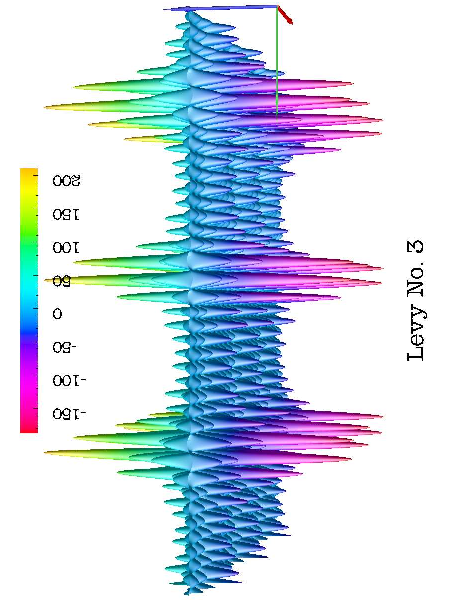
\includegraphics[width=0.5\textwidth,angle=-90]{figures/levy3}
\caption{\label{levy3} Levy No 3  \gref{levy3f}}
\end{center}
\end{figure}
%
\begin{figure}[!htb]
\begin{center}
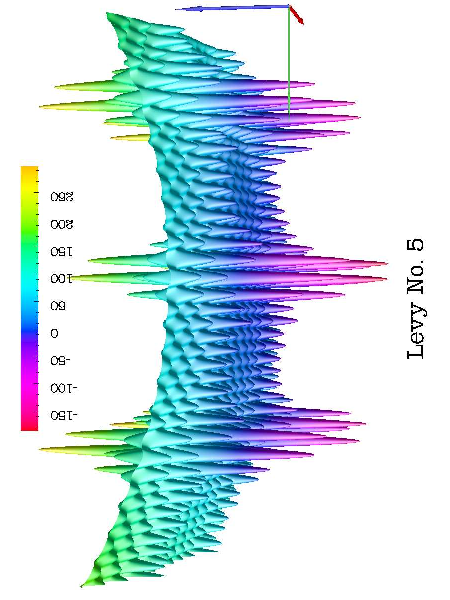
\includegraphics[width=0.5\textwidth,angle=-90]{figures/levy5}
\caption{\label{levy5} Levy No 5  \gref{levy5f}}
\end{center}
\end{figure}
\par{Levy No 5 function, see figure \gref{levy5},  has a global minimum
$-186.73090$  and about 760 local minima (2 dimensions) in the box
$-10.0\leq x_i \leq 10.0$ $i=\overline{1,2}$}
%
\be
\label{levy5f}
f(x)=\sum_{i=1}^{5}i\cos[(i+1)x_1+i]\sum_{j=1}^{5}j\cos[(j+1)x_2+j]+(x_1+1.42513)^2+(x_2+0.80032)^2
\ee
%
%
\par{Levy No 8 function, see figure \gref{levy8},  has a global minimum
$0$ at $(0,0,0 ...)$ in the box
$-10.0\leq x_i \leq 10.0$ $i=\overline{1,n}$}
%
\be
\label{levy8f}
f(x)=\sin^2(\pi y_1)+\sum_{i=1}^{n-1}(y_i-1)^2[1+10\sin^2(\pi y_{i+1})]+(y_n-1)^2
\ee
where $y_i=1+\frac{x_i-1}{4}$\\
%
\begin{figure}[!htb]
\begin{center}
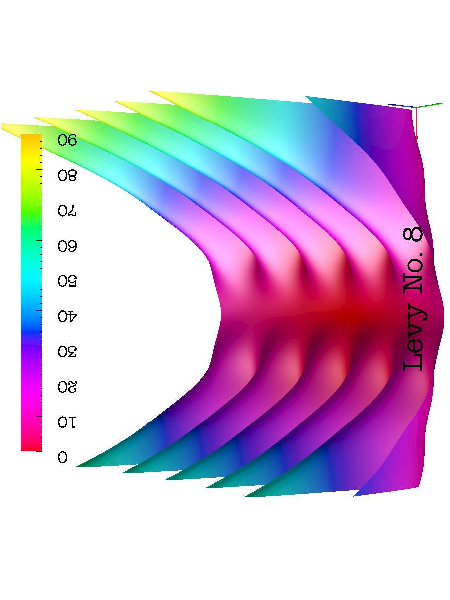
\includegraphics[width=0.5\textwidth,angle=-90]{figures/levy8}
\end{center}
\caption{Levy No 8  \gref{levy8f}}
\label{levy8}
\end{figure}
%
\begin{figure}[!htb]
\begin{center}
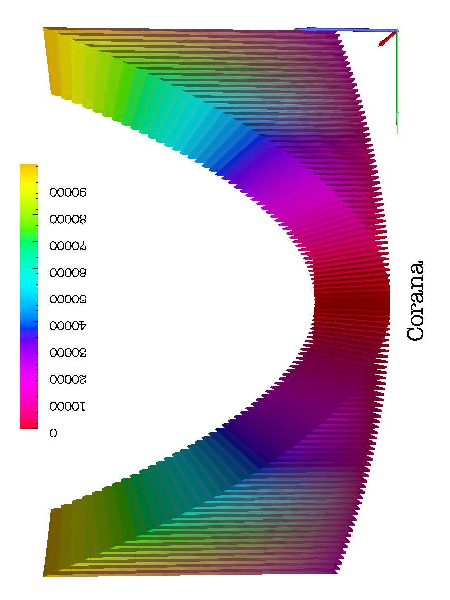
\includegraphics[width=0.5\textwidth,angle=-90]{figures/corana}
\caption{Corana  \gref{coranaf}}
\label{corana}
\end{center}
\end{figure}
%
\par{Corana function, proposed in \citep{Corana87} has a global minimum $0$ at $(0,0,0 ...)$ in the box
$-1000.0\leq x_i \leq 1000.0$ $i=\overline{1,n}$}
%
\be
\label{coranaf}
f(x)=\sum_{i=1}^n\left\{\begin{array}{ll}
(t_i\textrm{sgn}({z_i})+z_i)^2cd_i&\textrm{if }|x_i-z_i|<|t_i|\\
d_ix_i^2&\textrm{otherwise}
\end{array}\right.
\ee
where $z_i=\lfloor |x_i/s_i|+0.49999\rfloor\textrm{sgn}(x_i)s_i$, $s_i=0.2$,
$t_i=0.05$, $d_i=(1,1000,10,100, ...)$, $c=0.15$, $s_i,t_i,d_i$ repeated in cycles of 4, $c$ is a coefficient
defined in such a that \gref{coranaf} defines a paraboloid with axis parallel
to the coordinates, and a set of holes ($\lfloor x\rfloor$ is floor function
giving largest integer less than or equal to $x$), see Figure \gref{corana}.
\par{Rosenbrock function, see figure \gref{rosenbrock},  has a global minimum 0 at
$(1,1,1,...)$ in the box $-2.048\leq x_i \leq 2.048$ $i=\overline{1,n}$}
\be
\label{rosenbrockf}
f(x)=\sum_{i=1}^{n-1}100(x_{i+1}-x_i^2)^2+(1-x_i)^2
\ee
\begin{figure}[!htb]
\begin{center}
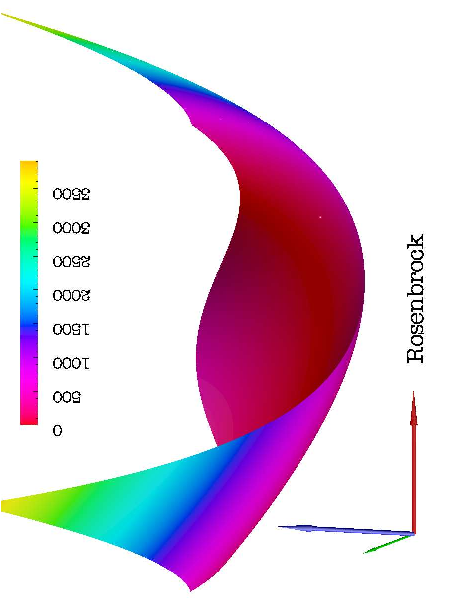
\includegraphics[width=0.5\textwidth,angle=-90]{figures/rosenbrock}
\end{center}
\caption{Rosenbrock  \gref{rosenbrockf}}
\label{rosenbrock}
\end{figure}
\begin{figure}[tb]
\begin{center}
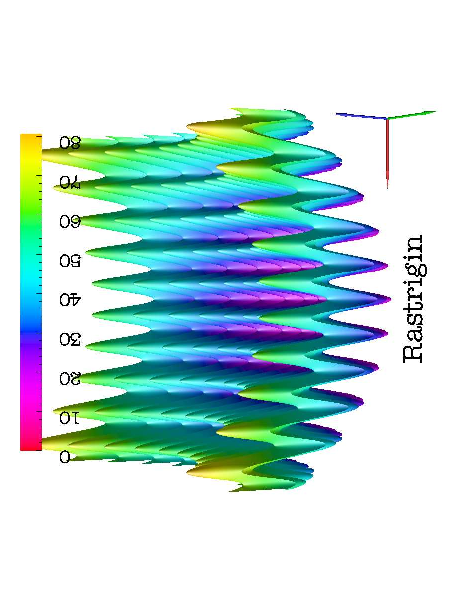
\includegraphics[width=0.5\textwidth,angle=-90]{figures/rastrigin}
\end{center}
\caption{Rastrigin  \gref{rastriginf} }
\label{rastrigin}
\end{figure}
\par{Rastrigin function, see figure \gref{rastrigin},  has a global minimum 0 at $(0,0,0,...)$ in the box
$-5.12\leq x_i \leq 5.12$ $i=\overline{1,n}$}
\be
\label{rastriginf}
f(x)=10n+\sum_{i=1}^{n}x_i^2-10\cos(2\pi x_i)
\ee
%
\par{Schwefel (Sine root) function, see figure \gref{schwefel},  has a global
minimum 0 at $(c,c,c,...)$ $c=420.9687464$ in the box
$-500\leq x_i \leq 500$ $i=\overline{1,n}$}
\be
\label{schwefelf}
f(x)=418.982887272433n-\sum_{i=1}^{n}x_i\sin(\sqrt{|x_i|})
\ee
\begin{figure}[!htb]
\begin{center}
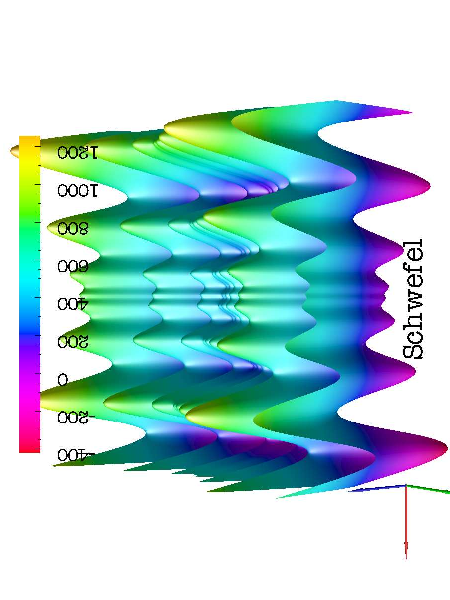
\includegraphics[width=0.5\textwidth,angle=-90]{figures/schwefel}
\end{center}
\caption{Schwefel  \gref{schwefelf}}
\label{schwefel}
\end{figure}
%
\begin{figure}[!htb]
\begin{center}
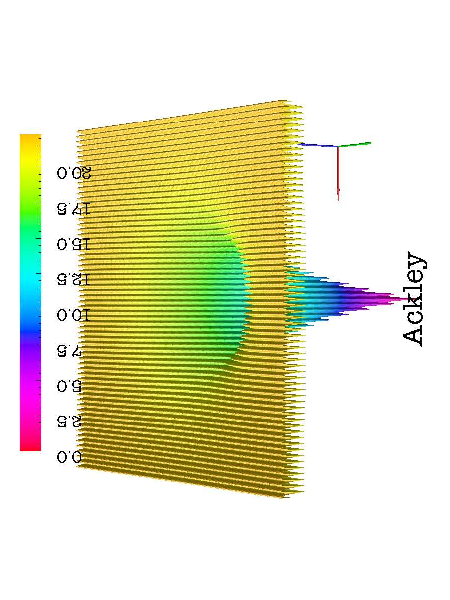
\includegraphics[width=0.5\textwidth,angle=-90]{figures/ackley}
\end{center}
\caption{Ackley  \gref{ackleyf}}
\label{ackley}
\end{figure}
\par{Ackley function, see figure \gref{ackley},  has a global minimum 0 at
$(0,0,0,...)$ in the box $-32.768\leq x_i \leq 32.768$ $i=\overline{1,n}$}
%
\be
\label{ackleyf}
f(x)=20+e-20\exp{\biggl[-0.2\sqrt{\frac{1}{n}\sum_{i=1}^{n}x_i^2}\biggr]}-\exp{\biggl[\frac{1}{n}\sum_{i=1}^{n}\cos(2\pi x_i)\biggr]}
\ee
%
%
\begin{table}[!htb]
\caption{Tests results}
\label{tabletest}
%\begin{spacing}{1.0}
\begin{center}
\begin{tabular}[h]{|l|r|r|r|r|r|r|r|}
\hline
Algorithm & \multicolumn{2}{|c|}{Simplex} & \multicolumn{2}{|c|}{SA} &
\multicolumn{3}{|c|}{SSA}\\
\hline
Function& $T_{CPU}$ & Hits & $T_{CPU}$ & Hits& $T_{CPU}$ & Hits1 & Hits2\\
\hline
\hline
\multicolumn{8}{|c|}{2 dimensions}\\
\hline
Levy no 3&5.56&1922&32.44&2000&74.70&1332&1999\\
\hline
Levy no 5&5.68&810&34.07&816&52.41&567&729\\
\hline
Levy no 8&4.69&2000&21.55&2000&66.97&983&2000\\
\hline
Corana&3.78&2000&24.17&2000&19.69&52&2000\\
\hline
Rosenbrock&4.28&2000&19.07&1995&53.06&896&2000\\
\hline
Rastrigin&4.31&988&14.66&1441&25.71&29&1348\\
\hline
Schwefel&4.56&1033&21.67&1983&39.56&636&1817\\
\hline
Ackley&5.47&2000&23.15&2000&97.09&1743&2000\\
\hline
\hline
\multicolumn{8}{|c|}{10 dimensions}\\
\hline
Levy no 8&568.76&9985&1322.59&10000&1884.03&1714&9988\\
\hline
Corana&495.86&9888&1186.01&9987&913.12&0&9895\\
\hline
Rosenbrock&313.29&8133&713.00&0&1690.20&7181&8246\\
\hline
Rastrigin&566.8626&2338&927.06&0&1581.78&0&2428\\
\hline
Schwefel&625.98&2879&1138.84&627&1598.23&0&2856\\
\hline
Ackley&499.62&9992&1005.59&10000&938.98&0&9989\\
\hline
\hline
\end{tabular}
\end{center}
%\end{spacing}
\end{table}
%
\section{Tight binding $N-H$, $N-N$ parameters}
\par{The fitting procedure described above was employed to solve the problem of
fitting the parameters for $N-H$ and $N-N$ bonds in a $NH_3$ and $N_2$
molecules. The parameters are from GSP-like scheme. The ``exact'' data are
represented by a hybrid DFT total energy curves. The basis set used to obtain them
was $6.31G(d,p)$ with the B3LYP functional. For $N_2$ the curve represents total energy vs $N-N$ bond length. For $NH_3$
two curves are investigated one is total energy vs $N-H$ bond length and the
second represents total energy vs $\theta$, where $\theta$ is defined as the
angle between $N-H$ bond direction and $C_3$ axis of symmetry, we refer about
the latter as ``umbrella'' curve. Table \gref{tablen2} summarise the parameters
for $N-N$ in $N_2$ molecule and Figure \gref{fitn2} shows the fit using our three
methods. The $N-H$ parameters for both modes are given in Table \gref{tablenh3}
and the fits are shown in figures \gref{fitnh3} and \gref{fitnh3um}.The zero
of energy is set to total energy of equilibrium geometry provided by hybrid
DFT calculations and the units are eV. The great majority of parameters from from Tables
\gref{tablen2} and \gref{tablenh3} lacks the physics due to the almost free
fitting strategy carried.}
\par{With the set of parameters provided by SSA method for $N-H$ bond we carried a
geometry optimisation using TDTB+UJ. The bond length was reproduced up to 0.008
{\AA} ($1.010$ {\AA} instead of $1.018$ \AA), but the bond angle was
underestimated ($88.7^\circ \approx 90^\circ$ instead of $105.7^\circ$). An
improvement could come adding $d$-orbitals, but we have not investigated
this option, yet. This lack of transferability of parameters
could come from the lack of physical insight put into the parameters
constraints. Figures \gref{spacenh3} and \gref{umbnh3} show us the surface of
the objective function in the space of two parameters, that we think could be
very important for the transferability of the model, $\epsilon_s$ (x
direction) and $\epsilon_p$ (y direction). The scanning is done in the box
$[-10.0,10.0]$ in an equal spaced grid of $201\times 201$. }
%
\begin{figure}[!htb]
\begin{center}
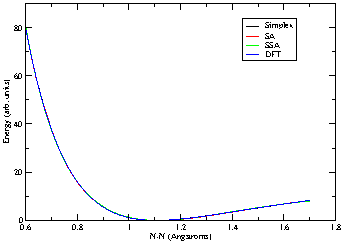
\includegraphics[width=0.75\textwidth]{figures/n2}
\end{center}
\caption{$N_2$ Energy fit}
\label{fitn2}
\end{figure}
%
\begin{figure}[!htb]
\begin{center}
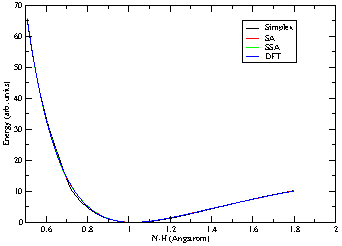
\includegraphics[width=0.75\textwidth]{figures/nh3}
\end{center}
\caption{$NH_3$ Energy fit}
\label{fitnh3}
\end{figure}
%
\begin{figure}
\begin{center}
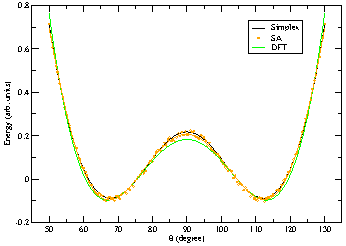
\includegraphics[width=0.75\textwidth]{figures/nh3u}
\caption{$NH_3$ ``Umbrella'' Energy fit}
\label{fitnh3um}
\end{center}
\end{figure}
%
\begin{figure}
\begin{center}
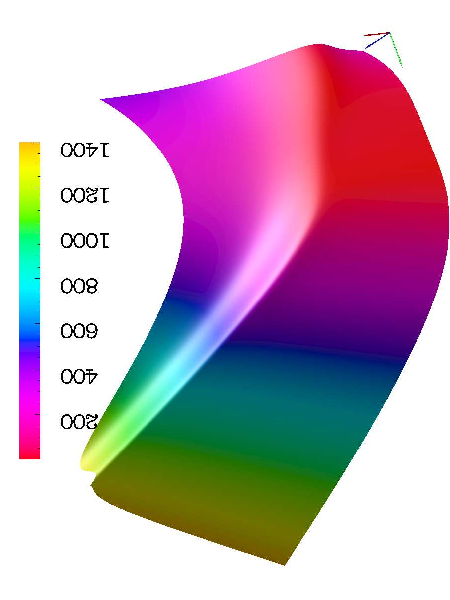
\includegraphics[width=0.5\textwidth,angle=-90]{figures/obj}
\caption{$NH_3$ Energy in $\epsilon_s$, $\epsilon_p$ space}
\label{spacenh3}
\end{center}
\end{figure}
%
\begin{figure}[!htb]
\begin{center}
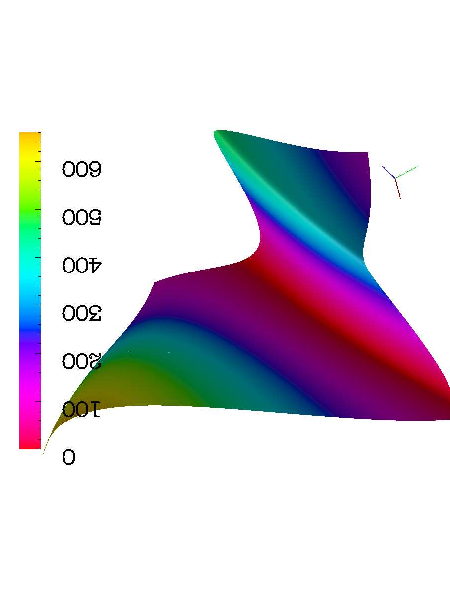
\includegraphics[width=0.5\textwidth,angle=-90]{figures/umbobj}
\caption{$NH_3$ ``Umbrella''Energy in $\epsilon_s$, $\epsilon_p$ space}
\label{umbnh3}
\end{center}
\end{figure}
%
%
%
\begin{table}[!thb]
\caption{$N-N$ $N_2$ parameters}
\label{tablen2}
\begin{center}
\begin{tabular}{|l|r|r|r|}
\hline
Parameter & Simplex & SA & SSA\\
\hline
\hline
$\epsilon_s$&-1.1952&-5.6667&-3.0500\\
\hline
$\epsilon_p$&4.4639&9.9550&1.0029\\
\hline
$\phi_0$&5.7837&8.8705&9.9991\\
\hline
$r_c$&1.3000&1.6913&1.5844\\
\hline
$n$&0.7689&1.5224&1.0531\\
\hline
$n_c$&2.5430&4.7195&3.8904\\
\hline
$d_0$&1.7141&1.1355&1.4432\\
\hline
$d_c$&1.9694&2.0393&1.9867\\
\hline
$m$&2.3991&3.5303&2.9362\\
\hline
$m_c$&5.5447&2.9813&8.2075\\
\hline
$ss\sigma$&8.5856&-9.2457&2.6236\\
\hline
$sp\sigma$&-8.3785& 0.8549&4.8730\\
\hline
$pp\sigma$&9.9148&4.6912&9.9552\\
\hline
$pp\pi$&9.5853&-2.7325&-3.9943\\
\hline
\end{tabular}
\end{center}
\end{table}
%
\begin{table}[!htb]
\caption{$N-H$ $NH_3$ parameters}
\label{tablenh3}
\begin{center}
\begin{tabular}{|l|r|r|r|r|r|r|}
\hline
Parameter &\multicolumn{3}{|c|}{E vs $N-H$}&\multicolumn{3}{|c|}{``Umbrella''}\\
\hline
 & Simplex & SA & SSA& Simplex & SA & SSA\\
\hline
\hline
$\epsilon_s$&-2.2488&-9.9999&-8.6831&-1.1757&-1.0057&-4.1313\\
\hline
$\epsilon_p$& 1.1181E-7&0.0&5.9505E-7&0.0&7.0686&9.1946\\
\hline
$\phi_0$&7.7089&7.2362&4.4385&5.0235&9.8324&7.4650\\
\hline
$r_c$&4.2321&2.3580&1.5000&1.8933&2.8450&2.8138\\
\hline
$n$&0.7201&0.2880&0.3728&0.7889&0.9057&1.1026\\
\hline
$n_c$&8.2522E-7&1.8152&4.2101&1.3140&5.3511& 2.5254\\
\hline
$d_0$&0.7686&0.7186&0.7615&0.8901&1.4739&1.2903\\
\hline
$d_c$&1.0799&1.1128&1.0761&1.3471&1.1100&1.5327\\
\hline
$m$&2.0893&2.5550&2.7400&1.0359&4.9930&3.0702\\
\hline
$m_c$&2.4259&3.2682&3.6451&2.8067&5.9471&5.9431\\
\hline
$ss\sigma$&0.5724&1.4376&-2.4421&3.9489&-9.9987&3.8607\\
\hline
$sp\sigma$&8.5354&9.5273& 4.1957&5.7663&-7.5378&8.9798E-5\\
\hline
\end{tabular}
\end{center}
\end{table}
 %
\section{Summary}
\par{We believe that the expressions we have given in \emph{Part Two} are suitable for
implementation in a TB-based molecular dynamics code. Though the expressions
are somewhat lengthy, they are well structured and can be coded by successive
function calls. The functions $A_{m}$, $B_{m}$, and $d^{l}_{mm^{\prime}}$ are expressed explicitly in the code, $S^{l}_{mm^{\prime}}$,
$T^{l}_{mm^{\prime}}$ and their derivatives with respect to $\alpha$ are implemented in terms of
these quantities. Derivatives with respect to $\beta$ are evaluated calling derivatives of the
Wigner $d$-function, which themselves are stated as combinations of Wigner
$d$-functions. Our approach goes further than \citep{Podolskiy04} adding the derivatives
of matrix elements and solves the problems at the poles ($\beta=0$). These have been already implemented in TDTB+UJ. A small paper
treating the topic was submitted, too.}
\par{The fitting procedure is of fundamental importance for a good work in our
project. Three methods were presented and investigated in \emph{Part Three}. The
simple implementation and the encouraging results in the testing phase made
them ideal candidates for our fitting problem. These methods are implemented
in TDTB+UJ to and they can be customised for use with different systems very
easy. Even if the parameters obtained for our test molecules $NH_3$ and $N_2$
are not fully satisfactory they have risen very useful questions to be
answered. Is it lack of physics in the parameters constraints or is the  model
chosen, non-self-consistent tight binding, not sufficient to address the
problem of PET molecules.}
\par{As a future development we hope that soon we will have a satisfactory time
dependent tight binding model for our Fluorescent PET sensors molecules. The
model should be able to explain the charge transfer in this molecules and a
set of transferable parameters should be obtained. }
\chapter[Push-pull]%
{Push-Pull Chromophores}
\label{ch:four}
%
 \chapterquote{to be decided, Maybe Poincare one}%
 {.....}
%


% appendices now
\begin{appendices}
\chapter[Spherical Harmonics]{Spherical Harmonics}
 \section[Complex Spherical ...]{Complex Spherical Harmonics}
\subsection{Definition}
 \par{A spherical harmonic $Y_{lm}(\vartheta,\varphi)$ is a single-valued function,
continuous, bounded complex function of two real arguments $\vartheta,\varphi$ with
$0\le \vartheta \le \pi$ and $0\le \varphi <2\pi$. It is characterised by the
parameters $l,m$, which take values $l=0,1,2,...$ and $|m| \le l$. Therefore, for
a given $l$ there are $2l+1$ functions corresponding to different $m$'s. All
derivatives of $Y_{lm}(\vartheta,\varphi)$ are single-valued, continuous and finite
functions.}
\subsection{Differential Equations}
\par{They are important in quantum physics. In fact they are eigenfunctions of
the operator of orbital angular quantum momentum and describe the angular
distribution of particles which move in a spherically-symmetric field with
orbital angular momentum $l$ and projection $m$. If ${\bf L}^2$ is the square
of orbital angular momentum and ${\bf L}_z$ the projection of orbital angular
momentum on the quantization axis we can write}
 
\begin{equation}
 \begin{split}
 {\bf L}^2Y_{lm}(\vartheta,\varphi)&=l(l+1)Y_{lm}(\vartheta,\varphi)\\
 {\bf L}_zY_{lm}(\vartheta,\varphi)&=mY_{lm}(\vartheta,\varphi)
 \end{split}
 \end{equation}
or in an expanded form
\begin{equation}
\label{sphdiff}
\begin{split}
\left[\frac{1}{\sin \vartheta}\p{}{\vartheta}\left(\sin \vartheta
    \p{}{\vartheta}\right)+\frac{1}{\sin^2
    \vartheta}\pp{}{\varphi}+l(l+1)\right]Y_{lm}(\vartheta,\varphi)&=0\\
\left[i\p{}{\varphi}+m\right]Y_{lm}(\vartheta,\varphi)&=0
\end{split}
\end{equation}
\par{Equations \gref{sphdiff} are invariant under the following transformations}
\begin{itemize}
\item $l\rightarrow \overline{l}=-l-1$
\item $\vartheta \rightarrow -\vartheta$ or $\vartheta \rightarrow
  \pi-\vartheta$
\item $m\rightarrow -m$
\item $\varphi \rightarrow -\varphi$
\end{itemize}
\subsection{Boundary Conditions}
\par{The first equation of \gref{sphdiff} is of second order. For fixed $l$ and $m$
it has two linear independent solutions. However, only one of them is regular,
satisfies the condition $|Y_{lm}(\vartheta,\varphi)|^2<\infty$ while the
other is singular at $\vartheta=0,\pi$. The regular solution satisfies the
following boundary conditions}
\begin{equation}
\label{boundary}
\begin{split}
Y_{lm}(\vartheta,\varphi \pm 2n\pi )&=Y_{lm}(\vartheta,\varphi)\\
\left.\p{}{\varphi}Y_{lm}(\vartheta,\varphi)\right|_{\vartheta=0}&=\left.\p{}{\varphi}Y_{lm}(\vartheta,\varphi)\right|_{\vartheta=\pi}=0
\end{split}
\end{equation}
\par{We shall consider only the spherical harmonics $Y_{lm}(\vartheta,\varphi)$
with $l$ and $m$ integers because the boundary conditions \gref{boundary} are
fulfilled only for such values of the parameters.}
\subsection[Normalization, Completeness ...]{Normalization, Completeness and other relations}
\par{The differential equations \gref{sphdiff} and the boundary conditions
  \gref{boundary} are homogeneous. Hence, they determine the spherical
  harmonics up to an arbitrary complex factor. The absolute value of this
  factor could be fixed by ortho-normalization relation}
\begin{equation}
\int_{0}^{2\pi}\td \varphi\int_{0}^{\pi}\td \vartheta \sin \vartheta Y_{l_1m_1}^{*}(\vartheta,\varphi)Y_{l_2m_2}(\vartheta,\varphi)=\delta_{l_1l_2}\delta_{m_1m_2}
\end{equation}
\par{The completeness relation for the spherical harmonics id given by}
\begin{equation}
\label{complet}
\sum_{l=0}^{\infty}\sum_{m=-l}^{m=l}Y_{lm}^{*}(\vartheta_1,\varphi_1)Y_{lm}(\vartheta_2,\varphi_2)=\delta(\varphi_1-\varphi_2)\delta(\cos
\vartheta_1-\cos \vartheta_2)
\end{equation}
\par{Sometimes instead of $Y_{lm}(\vartheta,\varphi)$ it is more convenient to
  use the function $C_{lm}(\vartheta,\varphi)$} which differs from
$Y_{lm}(\vartheta,\varphi)$ by the normalization factor
\begin{equation}
C_{lm}(\vartheta,\varphi)=\sqrt{\frac{4\pi}{2l+1}}Y_{lm}(\vartheta,\varphi) 
\end{equation}
\par{The function $C_{lm}(\vartheta,\varphi)$ satisfies the following relation}
\begin{equation}
\sum_{m}C_{lm}(\vartheta,\varphi)C_{lm}^{*}(\vartheta,\varphi)=1
\end{equation}
\par{The ortho-normalization relation is}
\begin{equation}
\int_{0}^{2\pi}\td \varphi\int_{0}^{\pi}\td \vartheta \sin \vartheta C_{l_1m_1}^{*}(\vartheta,\varphi)C_{l_2m_2}(\vartheta,\varphi)=\frac{2l+1}{4\pi}\delta_{l_1l_2}\delta_{m_1m_2}
\end{equation}
\subsection{Choice of Phase}
\par{An overall phase factor may be fixed by specifying the phase of one of the
harmonics $Y_{lm}(\vartheta,\varphi)$ for some given values of the arguments,
for example}
\begin{equation}
\label{y00}
Y_{l0}(0,0)=\sqrt{\frac{2l+1}{4\pi}} 
\end{equation}
\par{In this case the following relations are valid}
\begin{equation}
\label{ycomplex}
Y_{lm}^{*}(\vartheta,\varphi)=Y_{lm}(\vartheta,-\varphi)=(-1)^{m}Y_{l-m}(\vartheta,\varphi)
\end{equation}
\par{This choice of phase is known as Condon-Shortley phase convention and is
  very common in physics.}
\par{Equations \gref{sphdiff} and relations \gref{boundary}, \gref{y00},
  \gref{ycomplex} completely define $Y_{lm}(\vartheta,\varphi)$. Since $l$ and $m$ are integers,
  $Y_{lm}(\vartheta,\varphi)$ is single-valued.}
\subsection[Solutions of Some ...]{Solutions of Some Differential Equations in Terms of $Y_{lm}(\vartheta,\varphi)$}
\par{(a) Solution of Laplace equation}
\begin{equation}
\nabla^2f(r,\vartheta,\varphi)=0
\end{equation}
in polar coordinates is given by
\begin{equation}
R_{lm}(r,\vartheta,\varphi)=r^lY_{lm}(\vartheta,\varphi)\qquad I_{lm}(r,\vartheta,\varphi)=r^{(-l-1)}Y_{lm}(\vartheta,\varphi) 
\end{equation}
where $I_{lm}(r,\vartheta,\varphi)$ is irregular at $r=0$ and
$R_{lm}(r,\vartheta,\varphi)$ is regular. These functions are called solid
harmonics. In Cartesian coordinate representation $R_{lm}$ is a homogeneous
polynomial of degree $l$
\begin{equation}
r^lY_{lm}(\vartheta,\varphi)=\sqrt{\frac{2l+1}{4\pi}(l+m)!(l-m)!}\sum_{p,q,t}\frac{1}{p!q!t!}\left(-\frac{x+iy}{2}\right)^p\left(\frac{x-iy}{2}\right)^qz^t
\end{equation}
\par{Here $p,q,t$ are positive integers which satisfy $p+q+t=l$, $p-q=m$.}
\par{(b) Solution of the Helmholtz wave equation}
\begin{equation}
\left[\nabla^2+k^2\right]f(r,\vartheta,\varphi)=0
\end{equation}
\par{In polar coordinates may be expressed in terms of the function
$z_l(kr)Y_{lm}(\vartheta,\varphi)$ where
$z_l(kr)=\sqrt{\frac{\pi}{2kr}}Z_{l+1/2}(kr)$, $Z_{l+1/2}(kr)$ being any of
Bessel functions.}
\begin{equation}
L_{lm}^{r}(r,\vartheta,\varphi)=i^lj_l(kr)Y_{lm}(\vartheta,\varphi)\qquad L_{lm}^{i}(r,\vartheta,\varphi)=i^ln_l(kr)Y_{lm}(\vartheta,\varphi) 
\end{equation}
\par{$L_{lm}^{r}$ is regular at $r=0$, whereas $L_{lm}^{i}$ is irregular. These
functions are called standing spherical waves.}
\begin{equation}
B_{lm}^{(1)}(r,\vartheta,\varphi)=i^lh_l^{(1)}(kr)Y_{lm}(\vartheta,\varphi)\qquad B_{lm}^{(2)}(r,\vartheta,\varphi)=i^lh_l^{(2)}(kr)Y_{lm}(\vartheta,\varphi) 
\end{equation}
\par {$B_{lm}^{(1)}$ corresponds to a spherical wave which converges to origin, while
$B_{lm}^{(2)}$ corresponds to an outgoing spherical wave. These functions are
called running spherical waves. In the limit $k \rightarrow 0$ we regain
Laplace equation and solid harmonics.}
\subsection[Explicit form ...]{Explicit form of spherical harmonics}
\begin{equation}
Y_{lm}(\vartheta,\varphi)=e^{im\varphi}\sqrt{\frac{2l+1}{4\pi}\frac{(l-m)!}{(l+m)!}}P_l^m(\cos \vartheta)
\end{equation}
where $P_l^m(\cos \vartheta)$ associated Legendre polynomials.
\par{For special values of arguments and parameters we have}
\begin{equation}
Y_{lm}(0,\varphi)=\delta_{m0}\sqrt{\frac{2l+1}{4\pi}}
\end{equation}
\begin{equation}
Y_{lm}(\pi,\varphi)=\delta_{m0}(-1)^l\sqrt{\frac{2l+1}{4\pi}}
\end{equation}
\begin{equation}
Y_{lm}(\pm n\pi,\varphi)=\delta_{m0}(-1)^{nl}\sqrt{\frac{2l+1}{4\pi}}
\end{equation}
\begin{equation}
Y_{lm}(\frac{\pi}{2},\varphi)=\left\{\begin{array}{lc}
(-1)^{\frac{l+m}{2}}e^{im\varphi}\sqrt{\frac{2l+1}{4\pi}\cdot
  \frac{(l+m-1)!!}{(l+m)!!}\cdot \frac{(l-m-1)!!}{(l-m)!!}} & \text{if
}l+m\text{ is even}\\
0 & \text{if }l+m\text{ is odd}
\end{array}
\right.
\end{equation}
\subsection[Symmetry Properties ...]{Symmetry Properties and Other Relations}
\par{The symmetry relations given bellow couple spherical harmonics
  $Y_{lm}(\vartheta,\varphi)$ with different values of $\vartheta,\varphi$ and
  $l,m$.}
\begin{equation}
Y_{lm}^{*}(\vartheta,\varphi)=Y_{lm}(\vartheta,-\varphi)=(-1)^mY_{l-m}^{*}(\vartheta,\varphi)
\end{equation}
\begin{equation}
Y_{l-m}(\vartheta,\varphi)=(-1)^mY_{lm}(\vartheta,-\varphi)=(-1)^mY_{lm}^{*}(\vartheta,\varphi)=(-1)^me^{-i2m\varphi}Y_{lm}(\vartheta,\varphi)
\end{equation}
\begin{equation}
Y_{-l-1,m}(\vartheta,\varphi)=(-1)^mY_{lm}(\vartheta,\varphi)
\end{equation}
\begin{equation}
Y_{lm}(\pi-\vartheta,\varphi)=(-1)^{l+m}Y_{lm}(\vartheta,\varphi)
\end{equation}
\begin{equation}
Y_{lm}(\vartheta,\pi+\varphi)=(-1)^mY_{lm}(\vartheta,\varphi)
\end{equation}
\begin{equation}
Y_{lm}(\pi-\vartheta,\pi+\varphi)=(-1)^lY_{lm}(\vartheta,\varphi)
\end{equation}
\begin{equation}
Y_{lm}(-\vartheta,\varphi)=(-1)^mY_{lm}(\vartheta,\varphi)
\end{equation}
\begin{equation}
Y_{lm}(\vartheta,-\varphi)=(-1)^mY_{l-m}(\vartheta,\varphi)
\end{equation}
\begin{equation}
Y_{lm}(-\vartheta,-\varphi)=Y_{l-m}(\vartheta,\varphi)
\end{equation}
\begin{equation}
Y_{lm}(\vartheta \pm n\pi,\varphi)=\left\{ \begin{array}{lc}
(-1)^lY_{lm}(\vartheta,\varphi) & \text{if }n \text{ is odd}\\
Y_{lm}(\vartheta,\varphi) & \text{if }n \text{ is even}\\
\end{array}
\right.
\end{equation}
\begin{equation}
Y_{lm}(\vartheta,\varphi \pm n\pi)=\left\{ \begin{array}{lc}
(-1)^mY_{lm}(\vartheta,\varphi) & \text{if }n \text{ is odd}\\
Y_{lm}(\vartheta,\varphi) & \text{if }n \text{ is even}\\
\end{array}
\right.
\end{equation}
\par{Other useful relations could be}
\begin{equation}
\sum_{m} Y_{lm}(\vartheta,\varphi)Y_{lm}{*}(\vartheta,\varphi)=\frac{2l+1}{4\pi}
\end{equation}
\par{Proof is easy. We start with}
\begin{equation}
\sum_{m} Y_{lm}(\vartheta,\varphi)Y_{lm}{*}(\vartheta,\varphi)=I
\end{equation}
and then integrating over the angles and using the completeness relation we get
\begin{equation}
\begin{split}
\sum_{m}&=4I\pi\\
I&=\frac{2l+1}{4\pi}
\end{split}
\end{equation} 
\begin{equation}
\sum_{m} mY_{lm}(\vartheta,\varphi)Y_{lm}{*}(\vartheta,\varphi)=0
\end{equation}
\par{Following the same line as for the previous relation we get}
\begin{equation}
\begin{split}
\sum_{m=-l}^{l} m&=I\\
I&=0
\end{split}
\end{equation}
\par{A comprehensive description of complex spherical harmonics and their
  properties can be found in \citep{Varshalovich88}} 
%
\subsection[Expansion in Series ...]{Expansion in Series of the Spherical Harmonics}
%
\par{An arbitrary function $f(\vartheta,\varphi)$ which is defined in the interval $0\le \vartheta \le
\pi$ and $0\le \varphi <2\pi$ and satisfies the condition}
\begin{equation}
\int_{0}^{2\pi}\td \varphi \int_{0}^{\pi} \td \vartheta \sin \vartheta
|f(\vartheta,\varphi)|^2< \infty
\end{equation} 
can be expanded into a series of the spherical harmonics as
\begin{equation}
\label{multipole}
f(\vartheta,\varphi)=\sum_{l=0}^{\infty}\sum_{m=-l}^{m=l}a_{lm}Y_{lm}(\vartheta,\varphi)
\end{equation}
\par{The expansion coefficients $a_{lm}$ are given by the relation}
\begin{equation}
a_{lm}=\int_{0}^{2\pi}\td \varphi \int_{0}^{\pi} \td \vartheta \sin \vartheta Y_{lm}^{*}(\vartheta,\varphi)f(\vartheta,\varphi)
\end{equation}
\par{This relation may be treated as an integral transformation of
$f(\vartheta,\varphi)$ from the continuous variables $\vartheta,\varphi$ to
the discrete variables $l,m$.}
\par{The expansion coefficients $a_{lm}$ satisfy the Parceval condition}
\begin{equation}
\sum_{l=0}^{\infty}\sum_{m=-l}^{m=l}|a_{lm}|^2=\int_{0}^{2\pi}\td \varphi
\int_{0}^{\pi} \td \vartheta \sin \vartheta |f(\vartheta,\varphi)|^2
\end{equation}
\par{The expansion \gref{multipole} in terms of the spherical harmonics is
  widely used in different branches of physics. It is called the {\it
  multipole expansion}, and $a_{lm}$ are called {\it multipole moments}.}
\par{Two expansions are widely used in physics world}
\begin{equation}
\label{cwave}
e^{i{\bf k}\cdot {\bf R}}=4\pi
\sum_{l=0}^{\infty}\sum_{m=-l}^{l}i^lj_l(kR)Y_{lm}(\hat{\bf R})Y_{lm}^{*}(\hat{\bf k})
\end{equation}
\begin{equation}
\label{coulomb}
\frac{1}{|{\bf r}_1-{\bf r}_2|}=\sum_{l=0}^{\infty}\sum_{m=-l}^{l}\frac{4 \pi}{2l+1}\frac{r_<^l}{r_>^{l+1}}Y_{lm}(\hat{{\bf r}_2})Y_{lm}^{*}(\hat{{\bf r}_1})
\end{equation}
where $r_<=\min (r_1,r_2)$ and $r_>=\max (r_1,r_2)$, $\hat{\bf x}$ stands for
the angular dependence of ${\bf x}$. If $r_1<r_2$ we get
\begin{equation}
\begin{split}
\frac{1}{|{\bf r}_1-{\bf r}_2|}=&\sum_{l=0}^{\infty}\sum_{m=-l}^{l}\frac{4 \pi}{2l+1}\frac{r_1^l}{r_2^{l+1}}Y_{lm}(\hat{{\bf r}_2})Y_{lm}^{*}(\hat{{\bf r}_1})\\=&\sum_{l=0}^{\infty}\sum_{m=-l}^{l}(-1)^m\frac{4 \pi}{2l+1}R_{l-m}({\bf r}_1)I_{lm}({\bf r}_2)
\end{split}
\end{equation}
%
\subsection[Expansion of Products...]{Expansion of Products of the Spherical Harmonics}
\par{A direct product of two spherical harmonics of the same argument may be
  expanded in series as (the so-called {\it Clebsch-Gordan series})}
\begin{equation}
\label{product2}
Y_{l_1m_1}(\vartheta,\varphi)Y_{l_2m_2}(\vartheta,\varphi)=\sum_{L=0}^{\infty}\sum_{M=-L}^{L}\sqrt{\frac{(2l_1+1)(2l_2+1)}{4\pi(2L+1)}}C_{l_10l_20}^{L0}C_{l_1m_1l_2m_2}^{LM}Y_{LM}(\vartheta,\varphi)
\end{equation}
\par{The inverse relation may be written as}
\begin{equation}
\begin{split}
C_{l_10l_20}^{L0}Y_{LM}(\vartheta,\varphi)=&\sqrt{\frac{(2l_1+1)(2l_2+1)}{4\pi(2L+1)}}\\&\times\sum_{m_1=-l_1}^{l_1}\sum_{m_2=-l_2}^{l_2}C_{l_1m_1l_2m_2}^{LM}Y_{l_1m_1}(\vartheta,\varphi)Y_{l_2m_2}(\vartheta,\varphi)
\end{split}
\end{equation}
\par{Product of three spherical harmonics can be decomposed as}
\begin{equation}
\begin{split}
Y_{l_1m_1}(\vartheta,\varphi)Y_{l_2m_2}(\vartheta,\varphi)Y_{l_3m_3}(\vartheta,\varphi)=&\sum_{L,L^{\prime},M,M^{\prime}}\sqrt{\frac{(2l_1+1)(2l_2+1)(2l_3+1)}{(4\pi)^2(2L+1)}}\\&\times C_{l_10l_20}^{L^{\prime}0}C_{L^{\prime}0l_30}^{L0}
C_{l_1m_1l_2m_2}^{L^{\prime}M^{\prime}}C_{L^{\prime}M^{\prime}l_2m_2}^{LM}Y_{LM}(\vartheta,\varphi)
\end{split}
\end{equation}
\subsection[Integrals ...]{Integrals over Total Solid Angle}
\begin{equation}
\int_{0}^{2\pi}\td \varphi\int_{0}^{\pi}\td \vartheta \sin \vartheta Y_{lm}(\vartheta,\varphi)=\sqrt{4\pi}\delta_{l0}\delta_{m0}
\end{equation}
\par{To get the result we multiply the integrand by $Y_{00}^{*}(\vartheta,\varphi)$ and
divide it by the same quantity. Taking into account that
$1/Y_{00}^{*}(\vartheta,\varphi)=\sqrt{4\pi}$ and using completeness relation
we get our result.}
\begin{equation}
\int_{0}^{2\pi}\td \varphi\int_{0}^{\pi}\td \vartheta \sin \vartheta Y_{l_1m_1}(\vartheta,\varphi)Y_{l_2m_2}(\vartheta,\varphi)=(-1)^{m_2}\delta_{l_1l_2}\delta_{m_1-m_2}
\end{equation}
\par{We replace $Y_{l_2m_2}(\vartheta,\varphi)$ with
$(1)^{m_2}Y_{l_2-m_2}(\vartheta,\varphi)$ and using completeness relation we
get the result.}
%
\begin{equation}
\label{gauntdef}
\begin{split}
\int_{0}^{2\pi}\td \varphi\int_{0}^{\pi}\td \vartheta \sin \vartheta
&Y_{l_1m_1}(\vartheta,\varphi)Y_{l_2m_2}(\vartheta,\varphi)Y_{l_3m_3}^{*}(\vartheta,\varphi)=\\=&\sqrt{\frac{(2l_1+1)(2l_2+1)}{4\pi(2l_3+1)}} C_{l_10l_20}^{l_30}C_{l_1m_1l_2m_2}^{l_3m_3}
:=G_{l_1m_1l_2m_2}^{l_3m_3}
\end{split}
\end{equation}
\par{Relation \gref{gauntdef} defines Gaunt coefficient $G_{l_1m_1l_2m_2}^{l_3m_3}$.}
\par{Replacing $Y_{l_1m_1}(\vartheta,\varphi)Y_{l_2m_2}(\vartheta,\varphi)$ with
the expansion \gref{product2} and using completeness relation we get our result.}
\begin{equation}
\label{yjm3}
\begin{split}
\int_{0}^{2\pi}\td \varphi&\int_{0}^{\pi}\td \vartheta \sin \vartheta
Y_{l_1m_1}(\vartheta,\varphi)Y_{l_2m_2}(\vartheta,\varphi)Y_{l_3m_3}(\vartheta,\varphi)=\\=&\sqrt{\frac{(2l_1+1)(2l_2+1)(2l_3+1)}{4\pi}}
\tjm{l_1}{0}{l_2}{0}{l_3}{0}\tjm{l_1}{m_1}{l_2}{m_2}{l_3}{m_3}\\=&(-1)^{m_3}G_{l_1m_1l_2m_2}^{l_3-m_3}
\end{split}
\end{equation}
%
where $\binom{l_1\quad l_2\quad l_3}{m_1\quad m_2\quad m_3}$ is Wigner
$3jm$-symbol.To prove relation relation \gref{yjm3} we just replace
$Y_{l_3m_3}(\vartheta,\varphi)$ with
$(-1)^{m_3}Y_{l_3-m_3}^{*}(\vartheta,\varphi)$. Then we apply
relation \gref{gauntdef} and get our result.
%
\par{ The connection with Clebsch-Gordon coefficients is}
\begin{equation}
\tjm{j_1}{m_1}{j_2}{m_2}{j_3}{m_3}=(-1)^{j_3+m_3+2j_1}\frac{1}{\sqrt{2j_3+1}}C_{j_1-m_1j_2-m_2}^{j_3m_3}
\end{equation}
\par{The inverse relation is}
\begin{equation}
C_{j_1m_1j_2m_2}^{j_3m_3}=(-1)^{j_1-j_2+m_3}\sqrt{2j_3+1}\tjm{j_1}{m_1}{j_2}{m_2}{j_3}{-m_3}
\end{equation}
\par{The $3jm$-symbol represents the probability amplitude that three angular
momenta ${\bf j}_1,{\bf j}_3,{\bf j}_3$ with projections $m_1,m_2,m_3$ are
coupled to yields zero angular momentum}
\begin{equation}
\tjm{j_1}{m_1}{j_2}{m_2}{j_3}{m_3}=(-1)^{j_1-j_2+j_3}\sum_{jm}C_{j_1m_1j_2m_2}^{jm}C_{jmj_3m_3}^{00}
\end{equation}
%
\subsection{Solid Spherical Harmonics}
\par{Solid harmonics regular and irregular are solutions of laplace equation,
  hence their study is of a great interest. The addition theorems are}
\begin{equation}
R_{lm}(\bm{a}+\bm{b})=\sum_{l_1=0}^{l}\sum_{m=-l_1}^{l_1}\frac{4\pi(2l+1)!!}{(2l_1+1)!!(2l_2+1)!!}\mc{G}_{l_1m_1l_2m_2}^{lm}R_{l_1m_1}(\bm{a})R_{l_2m_2}(\bm{b})
\end{equation}
with $l=l_1+l_2$ and $m=m_1+m_2$
\begin{equation}
I_{lm}({\bf a}+\bm{b})=\sum_{l_1,m_1}\frac{4\pi(2l_1-1)!!}{(2l-1)!!(2l_2+1)!!}(-1)^{l_2}R_{l_2m_2}^{*}({\bf a})I_{l_1m_1}({\bm{b}})G_{lml_2m_2}^{l_1m_1}
\end{equation}
with $l_1=l+l_2$ and $m_1=m+m_2$
\par{The proofs of these theorems follow the line of \citep{Chakrabarti95},\citep{Deb83}.}
\par{\textbf{Regular solid harmonics. }
We start with expansion \gref{cwave}. We multiply it by $Y_{l_1m_1}(\hat{\bm{k}})$
and integrate over $\bm{k}$ angles. Using the orthonormality relation we get}
\begin{equation}
\begin{split}
\int \td {\hat{\bm{k}}}e^{i{\bf k}\cdot {\bf R}}Y_{l_1m_1}(\hat{\bm{k}})&=4\pi
\sum_{l=0}^{\infty}\sum_{m=-l}^{l}i^lj_l(kR)Y_{lm}(\hat{\bf R})\int \td
{\hat{\bm{k}}} Y_{lm}^{*}(\hat{\bf k})Y_{l_1m_1}(\hat{\bm{k}})\\
Q&=4\pi
\sum_{l=0}^{\infty}\sum_{m=-l}^{l}i^lj_l(kR)Y_{lm}(\hat{\bf R})\delta_{ll_1}\delta_{mm_1}
\end{split}
\end{equation}
\begin{equation}
\label{p1}
Q=4\pi i^lj_l(kR)Y_{lm}(\hat{\bf R})
\end{equation} 
where $Q$ stands for rihgt hand side and $\td {\hat{\bm{k}}}=\sin \vartheta
\td \vartheta \td \varphi$. Next, let us consider
$\bm{R}=\bm{a}+\bm{b}$ then we have $e^{i{\bf k}\cdot {\bf R}}=e^{i{\bf
    k}\cdot {\bf a}}e^{i{\bf k}\cdot {\bf b}}$ and inserting one expansion
\gref{cwave} for each exponential we get
\begin{equation}
\begin{split}
e^{i{\bf k}\cdot {\bf R}}=(4\pi)^2
\sum_{l_1=0}^{\infty}\sum_{m_1=-l_1}^{l_1}\sum_{l_2=0}^{\infty}\sum_{m_2=-l_2}^{l_2}i^{l_1+l_2}j_{l_1}(ka)j_{l_2}(kb)&Y_{l_1m_1}(\hat{\bf a})Y_{l_1m_1}^{*}(\hat{\bf k})\\&\times Y_{l_2m_2}(\hat{\bf b})Y_{l_2m_2}^{*}(\hat{\bf k})
\end{split}
\end{equation}
then multiplying it by $Y_{lm}(\hat{\bm{k}})$
and integrating over $\bm{k}$ angles we get
\begin{equation}
\label{p2}
Q=(4\pi)^2
\sum_{l_1=0}^{\infty}\sum_{m_1=-l_1}^{l_1}\sum_{l_2=0}^{\infty}i^{l_1+l_2}j_{l_1}(ka)j_{l_2}(kb)Y_{l_1m_1}(\hat{\bf a})Y_{l_2m_2}(\hat{\bf b})G_{l_1m_1l_2m_2}^{lm}
\end{equation}
with $G_{l_1m_1l_2m_2}^{lm}$ the Gaunt coefficient. Summation over $m_2$
disappers due to selection rule of Gaunt coefficients, $m_2=m-m_1$. $l$
obbeys the triangle inequality $|l_1-l_2|\le l\le |l_1+l_2|$. 
\par{Combining \gref{p1} with \gref{p2} we get}
\begin{equation}
i^lj_l(kR)Y_{lm}(\hat{\bf R})=4\pi\sum_{l_1=0}^{\infty}\sum_{m_1=-l_1}^{l_1}\sum_{l_2=0}^{\infty}i^{l_1+l_2}j_{l_1}(ka)j_{l_2}(kb)Y_{l_1m_1}(\hat{\bf a})Y_{l_2m_2}(\hat{\bf b})G_{l_1m_1l_2m_2}^{lm}
\end{equation}
using the behaviour of $j_l(kR)$ when $k\rightarrow 0$,
$j_l(kR)\xrightarrow{k\rightarrow 0}\frac{(kR)^l}{(2l+1)!!}$ we get
\begin{equation}
\frac{i^lR^{l}}{(2l+1)!!}Y_{lm}(\hat{\bf R})=4\pi\sum_{l_1=0}^{\infty}\sum_{m_1=-l_1}^{l_1}\sum_{l_2=0}^{\infty}\frac{i^{l_1+l_2}k^{l_1+l_2-l}a^{l_1}b^{l_2}}{(2l_1+1)!!(2l_2+1)!!}Y_{l_1m_1}(\hat{\bf a})Y_{l_2m_2}(\hat{\bf b})G_{l_1m_1l_2m_2}^{lm}
\end{equation}
and because in the limit  $k\rightarrow 0$ left hand side should be always
finite we get $l=l_1+l_2$ and relation becomes
\begin{equation*}
R_{lm}(\bm{R})=R_{lm}(\bm{a}+\bm{b})=4\pi\sum_{l_1=0}^{l}\sum_{m_1=-l_1}^{l_1}\frac{(2l+1)!!}{(2l_1+1)!!(2l_2+1)!!}R_{l_1m_1}({\bf a})R_{l_2m_2}({\bf b})G_{l_1m_1l_2m_2}^{lm}    
\end{equation*}
with $l_2=l-l_1$ and $m_2=m-m_1$ this is the addition theorem for regular
spherical harmonics.
\par{We also could find useful the following properties}
\begin{equation}
\begin{split}
R_{lm}(-\bm{r})&=r^lY_{lm}(\pi
-\vartheta,\pi+\varphi)=(-1)^{l}r^lY_{lm}(\vartheta,\varphi)=(-1)^lR_{lm}(\bm{r})\\
R_{lm}^{*}(r)&=r^lY_{lm}^{*}(\vartheta,\varphi)=(-1)^mr^lY_{l-m}(\vartheta,\varphi)=(-1)^mR_{l-m}(r)
\end{split}
\end{equation}
\par{\textbf{Irregular solid harmonics.} To prove the addition theorem for irregular solid harmonics we use
  expansion \gref{coulomb}(with the assumption $r_1<r_2$). We multiply it by
  $Y_{l_1m_1}(\hat{\bm{r}_1})$ and integrate over $\bm{r}_1$ angles. Using the
  orthonormality relation for spherical harmonics we get}
\begin{equation}
\begin{split}
\int \td \hat{\bm {r}_1} \frac{Y_{l_1m_1}(\hat{{\bf r}_1})}{|{\bf r}_1-{\bf
  r}_2|}&=\sum_{l=0}^{\infty}\sum_{m=-l}^{l}\frac{4
  \pi}{2l+1}\frac{r_1^l}{r_2^{l+1}}Y_{lm}(\hat{{\bf r}_2})\int \td \hat{\bm
  {r}_1} Y_{l_1m_1}(\hat{{\bf r}_1})Y_{lm}^{*}(\hat{{\bf r}_1})\\
Q&=\sum_{l=0}^{\infty}\sum_{m=-l}^{l}\frac{4
  \pi}{2l+1}\frac{r_1^l}{r_2^{l+1}}Y_{lm}(\hat{{\bf r}_2})\delta_{ll_1}\delta_{mm_1}
\end{split}
\end{equation}
\begin{equation}
\label{q1}
Q=\frac{4
  \pi}{2l+1}\frac{r_1^l}{r_2^{l+1}}Y_{lm}(\hat{{\bf r}_2})=\frac{4
  \pi}{2l+1}r_1^lI_{lm}({\bf r}_2)
\end{equation}
where $Q$ stands for the right hand side of the first line.
\par{Next let us consider $\bm{r}_2=\bm{a}+\bm{b}$, we assume that
  $|r_1-a|<b$}. In this conditions we get the following expansion
\begin{equation}
\frac{1}{|{\bf r}_1-{\bf r}_2|}=\frac{1}{|(\bm{r}_1-\bm{a})-\bm{b}|}=\sum_{l_1,m_1}\frac{4\pi}{2l_1+1}R_{l_1m_1}^{*}(\bm{r}_1-\bm{a})I_{l_1m_1}({\bm{b}})
\end{equation}
we used the definition of regular and irregular solid harmonics to write the
above relation in a condensed way. Next we apply addition theorem
for regular solid harmonics and we get
\begin{equation}
\begin{split}
\frac{1}{|(\bm{r}_1-\bm{a})-\bm{b}|}=\sum_{l_1,m_1}I_{l_1m_1}({\bm{b}})\sum_{l_2=0}^{l_1}\sum_{m_2=-l_2}^{l_2}&\frac{(4\pi)^2(2l_1-1)!!r_1^{l_2}}{(2l_2+1)!!(2l_3+1)!!}Y_{l_2m_2}^{*}(\hat{{\bf r}_1})\\&\times (-1)^{l_3}R_{l_3m_3}^{*}({\bf a})G_{l_2m_2l_3m_3}^{l_1m_1}
\end{split}
\end{equation}
\par{Multiplying it by $Y_{lm}(\hat{{\bf r}_1})$, integrating over ${\bf r}_1$
angles and finally using the orthonormality relation for spherical harmonics
we get}
\begin{equation}
\label{q2}
Q=\sum_{l_1,m_1}I_{l_1m_1}({\bm{b}})\frac{(4\pi)^2(2l_1-1)!!}{(2l+1)!!(2l_3+1)!!}(r_1)^{l}(-1)^{l_3}R_{l_3m_3}^{*}({\bf a})G_{lml_3m_3}^{l_1m_1}
\end{equation}
with $l_1=l+l_3$ and $m_1=m+m_3$
\par{Combining \gref{q1} with \gref{q2} we get}
\begin{equation}
\frac{1}{2l+1}r_1^lI_{lm}({\bf r}_2)=\sum_{l_1,m_1}I_{l_1m_1}({\bm{b}})\frac{4\pi(2l_1-1)!!}{(2l+1)!!(2l_3+1)!!}r_1^{l}(-1)^{l_3}R_{l_3m_3}^{*}({\bf a})G_{lml_3m_3}^{l_1m_1}
\end{equation}
and equating the coefficients of ${r}_1^{l}$
\begin{equation*}
I_{lm}({\bf r}_2)=I_{lm}({\bf a}+\bm{b})=\sum_{l_1,m_1}\frac{4\pi(2l_1-1)!!}{(2l-1)!!(2l_3+1)!!}(-1)^{l_3}R_{l_3m_3}^{*}({\bf a})I_{l_1m_1}({\bm{b}})G_{lml_3m_3}^{l_1m_1}
\end{equation*}
which is the addition theorem for irregular solid harmonics. The theorem was
obtained under some restrictions, but is very simple to prove it if we state the
opposite of this conditions following the same line.
\par{Following properties are useful}
\begin{equation}
\begin{split}
I_{lm}(-\bm{r})&=(-1)^lI_{lm}(\bm{r})\\
I_{lm}^{*}(\bm{r})&=(-1)^mI_{l-m}(\bm{r})
\end{split}
\end{equation} 
\section[Real Spherical ...]{Real Spherical Harmonics}
\subsection{Definition}
\par{We can define real spherical harmonics as}
\begin{equation}
\begin{split}
X_{l0}&:=Y_{l0}\\ m>0:\quad
X_{lm}&:=\sqrt{2}(-1)^m\text{Re}Y_{lm}\\m<0:\quad X_{lm}&:=\sqrt{2}(-1)^m\text{Im}Y_{l-m}
\end{split}\end{equation}
or in a condensed form
\begin{equation}
\label{Rspherdef}
X_{l\mu}(\vartheta,\varphi)=\sum_{m=-l}^{l}U_{lm}^{\mu}Y_{lm}(\vartheta,\varphi)
\end{equation}
where $\mu=\overline{-l...l}$, $U_{lm}^{\mu}$ represents a $(2l+1)\times (2l+1)$
unitary matrix for a fixed $l$ and has the
elements
\begin{equation}
U_{lm}^{\mu}=\delta_{m0}\delta_{\mu 0}+\frac{1}{\sqrt{2}}\left((-1)^m
  \Theta(\mu)\delta_{m\mu}+i\Theta(-\mu)\delta_{m\mu}-i(-1)^m \Theta(-\mu)\delta_{m-\mu}+\Theta(\mu)\delta_{m-\mu}\right)
\end{equation}
\par{$\Theta(\mu)$} is given by
\begin{equation}
\Theta(\mu)=\left\{\begin{array}{ll}
1&\textrm{if \(\mu>0\)}\\
0&\textrm{if \(\mu \le 0\)}
\end{array}\right.
\end{equation}
%
\par{We have}
\begin{equation}
\label{unit}
\sum_{m}[U_{lm}^{\mu}]^{*}U_{lm}^{\mu^{\prime}}=\delta_{\mu \mu^{\prime}}\qquad\sum_{\mu}[U_{lm}^{\mu}]^{*}U_{lm^{\prime}}^{\mu}=\delta_{m m^{\prime}}
\end{equation}
\par{The inverse relation of \gref{Rspherdef} is}
\begin{equation}
Y_{lm}(\vartheta,\varphi)=\sum_{\mu}[U_{lm}^{\mu}]^{*}X_{l\mu}(\vartheta,\varphi)
\end{equation}
\subsection{Useful Properties}
\par{Starting with obvious equality $[X_{l\mu}]^{*}=X_{l\mu}$ and expanding each
side in terms of \gref{Rspherdef} we get}
\begin{equation*}
\sum_{m=-l}^{l}U_{lm}^{\mu}Y_{lm}(\vartheta,\varphi)=\sum_{m=-l}^{l}[U_{lm}^{\mu}]^{*}Y_{lm}^{*}(\vartheta,\varphi)
\end{equation*}
\begin{equation}
\sum_{m=-l}^{l}\left\{(-1)^m[U_{l-m}^{\mu}]^{*}-U_{lm}^{\mu}\right\}Y_{lm}(\vartheta,\varphi)=0
\end{equation}
\par{Since the spherical harmonics are linearly independent for a fixed $l$ the
content of the curly brackets should vanish, so we get}
\begin{equation}
\label{ulm}
U_{lm}^{\mu}=(-1)^m[U_{l-m}^{\mu}]^{*}\qquad[U_{lm}^{\mu}]^{*}=(-1)^mU_{l-m}^{\mu}
\end{equation}
\par{A very useful relation is}
\begin{equation}
\label{sumxx}
\sum_{\mu}X_{l\mu}(\vartheta_1,\varphi_1)X_{l\mu}(\vartheta_2,\varphi_2)=\sum_{m}Y_{lm}(\vartheta_1,\varphi_1)Y_{lm}^{*}(\vartheta_2,\varphi_2)
\end{equation}
\par{The proof is straightforward. In left hand side we insert for each real
spherical harmonic an expansion \gref{Rspherdef} and we get}
\begin{equation}
\begin{split}
\sum_{\mu}X_{l\mu}(\vartheta_1,\varphi_1)&X_{l\mu}(\vartheta_2,\varphi_2)=\sum_{\mu}\sum_{m}U_{lm}^{\mu}Y_{lm}(\vartheta_1,\varphi_1)\sum_{m^{\prime}}U_{lm^{\prime}}^{\mu}Y_{lm^{\prime}}(\vartheta_2,\varphi_2)\\
&=\sum_{m}\sum_{m^{\prime}}(-1)^{m\prime}\sum_{\mu}[U_{l-m^{\prime}}^{\mu}]^{*}U_{lm}^{\mu}Y_{lm}(\vartheta_1,\varphi_1)Y_{lm^{\prime}}(\vartheta_2,\varphi_2)\\
&=\sum_{m}\sum_{m^{\prime}}(-1)^{m\prime}\delta_{m-m^{\prime}}Y_{lm}(\vartheta_1,\varphi_1)Y_{lm^{\prime}}(\vartheta_2,\varphi_2)\\&=\sum_{m}Y_{lm}(\vartheta_1,\varphi_1)Y_{lm}^{*}(\vartheta_2,\varphi_2)
\end{split}
\end{equation}
\par{To get second line we use \gref{ulm} and then in second we make use of
\gref{unit} and then using phase convention for spherical harmonics we get
right hand side of \gref{sumxx}.}
\par{The ortho-normalization relation for real spherical harmonics is easy to
  get.}
\begin{equation}
\begin{split}
\int_{0}^{2\pi}\td \varphi&  \int_{0}^{\pi}\td \vartheta \sin \vartheta
X_{l\mu}(\vartheta,\varphi)X_{l_1\mu_1}(\vartheta,\varphi)\\&=\sum_{m,m_1}U_{lm}^{\mu}U_{l_1m_1}^{\mu_1}\int_{0}^{2\pi}\td
\varphi \int_{0}^{\pi}\td \vartheta \sin \vartheta
Y_{lm}(\vartheta,\varphi)Y_{l_1m_1}(\vartheta,\varphi)\\
&=\sum_{m,m_1}U_{lm}^{\mu}U_{l_1m_1}^{\mu_1}(-1)^m\int_{0}^{2\pi}\td
\varphi \int_{0}^{\pi}\td \vartheta \sin \vartheta Y_{l-m}^{*}(\vartheta,\varphi)Y_{l_1m_1}(\vartheta,\varphi)\\&=\delta_{l,l_1}\sum_{m,m_1}U_{lm}^{\mu}U_{l_1m_1}^{\mu_1}(-1)^m\delta_{-m,m_1}=\delta_{l,l_1}\sum_{m}U_{lm}^{\mu}U_{l-m}^{\mu_1}(-1)^m\\&=\delta_{l,l_1}\sum_{m}U_{lm}^{\mu}[U_{lm}^{\mu_1}]^{*}=\delta_{l,l_1}\delta_{\mu,\mu_1}
\end{split}
\end{equation}
\par{In first line we replace each real spherical harmonics by an expansion
\gref{Rspherdef}. In second line we create the ortho-normalization relation for
complex spherical harmonics using phase convention relation. In forth line we
made use of \gref{unit} and we get our final result. The real spherical
harmonics keep the same form as complex one for the ortho-normalization
relation. Next let us check the completeness relation}
\begin{equation}
\begin{split}
\sum_{l,\mu}X_{l\mu}(\vartheta_1,\varphi_1)&X_{l\mu}(\vartheta_2,\varphi_2)=\sum_{l,\mu,m_1,m_2}U_{lm_1}^{\mu}U_{lm_2}^{\mu}Y_{lm_1}(\vartheta_1,\varphi_1)Y_{lm_2}(\vartheta_2,\varphi_2)\\&=\sum_{l,m_1,m_2}\sum_{\mu}[U_{l-m_1}^{\mu}]^{*}U_{lm_2}^{\mu}Y_{l-m_1}^{*}(\vartheta_1,\varphi_1)Y_{lm_2}(\vartheta_2,\varphi_2)\\&=\sum_{l,m_1,m_2}\delta_{-m_1,m_2}Y_{l-m_1}^{*}(\vartheta_1,\varphi_1)Y_{lm_2}(\vartheta_2,\varphi_2)\\&=\sum_{l,m}Y_{lm}^{*}(\vartheta_1,\varphi_1)Y_{lm}(\vartheta_2,\varphi_2)=\delta(\varphi_1-\varphi_2)\delta(\cos \vartheta_1-\cos \vartheta_2)
\end{split}
\end{equation}
\par{The line of proof is identical with that one followed for ortho-normalization relation.}
\subsection[Expansions ...]{Expansions in terms of real spherical harmonics}
\begin{equation}
\frac{1}{|{\bf r}_1-{\bf
    r}_2|}=\sum_{l=0}^{\infty}\sum_{m=-l}^{l}\frac{4\pi}{2l+1}\frac{r_<^l}{r_>^{l+1}}Y_{lm}(\hat{{\bf r}_1})Y_{lm}^{*}(\hat{{\bf r}_2})
\end{equation}
with $r_<=\min (r_1,r_2)$ and $r_>=\max (r_1,r_2)$.
\begin{equation}
\begin{split}
\frac{1}{|{\bf r}_1-{\bf
    r}_2|}&=\sum_{l=0}^{\infty}\sum_{m=-l}^{l}\frac{4\pi}{2l+1}\frac{r_<^l}{r_>^{l+1}}Y_{lm}(\hat{{\bf
    r}_1})Y_{lm}^{*}(\hat{{\bf r}_2})\\
&=\sum_{l=0}^{\infty}\sum_{m=-l}^{l}\frac{4\pi}{2l+1}\frac{r_<^l}{r_>^{l+1}}\sum_{\mu_1}\left[
    U_{lm}^{\mu_1}\right]^{*}X_{l\mu_1}(\hat{{\bf r}_1})\sum_{\mu_2}
    U_{lm}^{\mu_2}X_{l\mu_2}(\hat{{\bf r}_2})\\
&=\sum_{l=0}^{\infty}\frac{4\pi}{2l+1}\frac{r_<^l}{r_>^{l+1}}\sum_{\mu_1,\mu_2}\underbrace{\sum_{m=-l}^{l}\left[
    U_{lm}^{\mu_1}\right]^{*}U_{lm}^{\mu_2}}_{\delta_{\mu_1\mu_2}}X_{l\mu_1}(\hat{{\bf r}_1})X_{l\mu_2}(\hat{{\bf r}_2})
\end{split}
\end{equation}
\par{In the second line we replaced the complex spherical harmonics with expansions
in terms of the real counterparts. In the third line we use relation
\gref{unit} and we get the expansion}
\begin{equation}
\label{rcoulomb}
\frac{1}{|{\bf r}_1-{\bf
    r}_2|}=\sum_{l=0}^{\infty}\sum_{m=-l}^{l}\frac{4\pi}{2l+1}\frac{r_<^l}{r_>^{l+1}}X_{lm}(\hat{{\bf
    r}_1})X_{lm}(\hat{{\bf r}_2})
\end{equation}
for $r_1<r_2$ we have
\begin{equation}
 \frac{1}{|{\bf r}_1-{\bf
    r}_2|}=\sum_{l=0}^{\infty}\sum_{m=-l}^{l}\frac{4\pi}{2l+1}\mc{R}_{lm}({\bf
    r}_1)\mc{I}_{lm}({\bf r}_2)
\end{equation}
and for $r_1>r_2$
\begin{equation}
 \frac{1}{|{\bf r}_1-{\bf
    r}_2|}=\sum_{l=0}^{\infty}\sum_{m=-l}^{l}\frac{4\pi}{2l+1}\mc{I}_{lm}({\bf
    r}_1)\mc{R}_{lm}({\bf r}_2)
\end{equation}
where we defined $\mc{R}_{lm}$ and $\mc{I}_{lm}$ as
\begin{equation}
\mc{R}_{lm}({\bf r})=r^lX_{lm}(\hat{{\bf r}})\qquad \mc{I}_{lm}({\bf r})=r^{-l-1}X_{lm}(\hat{{\bf r}})
\end{equation}
\begin{equation}
e^{i\bm{r}_1\cdot\bm{r}_2}=4\pi\sum_{l=0}^{\infty}\sum_{m=-l}^{l}i^lj_l(r_1r_2)Y_{lm}(\hat{\bm{r}}_2)Y_{lm}^{*}(\hat{\bm{r}}_1)
\end{equation}
and following the same line as above we find out the following expansion
\begin{equation}
\label{rwave}
e^{i\bm{r}_1\cdot\bm{r}_2}=4\pi\sum_{l=0}^{\infty}\sum_{m=-l}^{l}i^lj_l(r_1r_2)X_{lm}(\hat{\bm{r}}_2)X_{lm}(\hat{\bm{r}}_1)
\end{equation}
\subsection[Addition Theorem ...]{Addition Theorem for Real Solid Harmonics}
\par{Relation \gref{rwave} could be used to get an addition theorem for
  $\mc{R}_{lm}$ as suggested in \citep{Chakrabarti95},\citep{Deb83}}
\par{Multiplying relation \gref{rwave} by $X_{l_1m_1}(\hat{\bm{r}}_1)$ and
  integrating over $\td \hat{\bm{r}}_1$ we get}
\begin{equation}
\label{part1}
\begin{split}
Q&=\int \td \hat{\bm{r}}_1
e^{i\bm{r}_1\cdot\bm{r}_2}X_{l_1m_1}(\hat{\bm{r}}_1)=4\pi\sum_{l=0}^{\infty}\sum_{m=-l}^{l}i^lj_l(r_1r_2)X_{lm}(\hat{\bm{r}}_2)\int \td \hat{\bm{r}}_1
X_{lm}(\hat{\bm{r}}_1)X_{l_1m_1}(\hat{\bm{r}}_1)\\
Q&=4\pi\sum_{l=0}^{\infty}\sum_{m=-l}^{l}i^lj_l(r_1r_2)X_{lm}(\hat{\bm{r}}_2)\delta_{ll_1}\delta_{mm_1}\\
Q&=4\pi i^lj_l(r_1r_2)X_{lm}(\hat{\bm{r}}_2)
\end{split}
\end{equation}
\par{Considering $\bm{r}=\bm{a}+\bm{b}$ we get
$e^{i\bm{r}_1\cdot\bm{r}_2}=e^{i\bm{r}_1\cdot\bm{a}}e^{i\bm{r}_1\cdot\bm{b}}$
and inserting an expansion \gref{rwave} for each exponential, and then,
multiplying relation by $X_{lm}(\hat{\bm{r}}_1)$ and integrating over $\td \hat{\bm{r}}_1$ we get}
\begin{equation}
\begin{split}
e^{i\bm{r}_1\cdot(\bm{a}+\bm{b})}=(4\pi)^2\sum_{l_1,m_1}i^{l_1}j_{l_1}(r_1a)X_{l_1m_1}(\hat{\bm{a}})X_{l_1m_1}(\hat{\bm{r}}_1)\sum_{l_2,m_2}i^{l_2}j_{l_2}(r_1b)X_{l_2m_2}(\hat{\bm{b}})X_{l_2m_2}(\hat{\bm{r}}_1)\\
Q=\sum_{\begin{subarray}{l}l_1,m_1\\
l_2,m_2
\end{subarray}
}i^{l_1+l_2}j_{l_1}(r_1a)j_{l_2}(r_1b)X_{l_1m_1}(\hat{\bm{a}})X_{l_2m_2}(\hat{\bm{b}})\int
\td \hat{\bm{r}}_1 X_{l_1m_1}(\hat{\bm{r}}_1)X_{l_2m_2}(\hat{\bm{r}}_1)X_{lm}(\hat{\bm{r}}_1)
\end{split}
\end{equation}
\par{The integral is nothing else than Gaunt coefficient for real spherical
  harmonics $\mc{G}_{l_1m_1l_2m_2}^{lm}=\int \td \hat{\bm{r}}_1
  X_{l_1m_1}(\hat{\bm{r}}_1)X_{l_2m_2}(\hat{\bm{r}}_1)X_{lm}(\hat{\bm{r}}_1)$.
  Using }
\begin{equation}
j_l(r_1r_2)\xrightarrow{r_1\rightarrow 0}\frac{(r_1r_2)^l}{(2l+1)!!}
\end{equation}
and replacing $Q$ with relation \gref {part1} we get
\begin{equation}
i^l(r_1r_2)^l=\sum_{\begin{subarray}{l}l_1,m_1\\
l_2,m_2
\end{subarray}}i^{l_1+l_2}\frac{4\pi(2l+1)!!}{(2l_1+1)!!(2l_2+1)!!}
r_1^{l_1+l_2}a^{l_1}X_{l_1m_1}(\hat{\bm{a}})b^{l_2}X_{l_2m_2}(\hat{\bm{b}})\mc{G}_{l_1m_1l_2m_2}^{lm}
\end{equation}
\par{Using the selection rules for real Gaunt coefficients and the fact that the
expansion should be finite, $m_2=m-m_1$ and $l_2=l-l_1$, we extract from above
expansion the addition rule for $\mc{R}_{lm}$}
\begin{equation}
\label{radd}
\mc{R}_{lm}(\bm{a}+\bm{b})=\sum_{l_1=0}^{l}\sum_{m_1=-l_1}^{l_1}\mc{G}_{l_1m_1l_2m_2}^{lm}\frac{4\pi(2l+1)!!}{(2l_1+1)!!(2l_2+1)!!}\mc{R}_{l_1m_1}(\bm{a})\mc{R}_{l_2m_2}(\bm{b})
\end{equation}
\par{ A similar theorem could be obtained for real irregular solid
  harmonics. We start with expansion \gref{rcoulomb}, for $r_1<r_2$ and
  multiplying it by $X_{l_1m_1}(\hat{\bm{r}_1})$, integrating over $\bm{r}_1$
  angles and using orthonormality relation for real spherical harmonics we
  get} 
\begin{equation}
\label{q4}
\begin{split}
\int \td \hat{\bm{r}}_1\frac{X_{l_1m_1}(\hat{\bm{r}_1})}{|{\bf r}_1-{\bf
    r}_2|}&=\sum_{l=0}^{\infty}\sum_{m=-l}^{l}\frac{4\pi}{2l+1}\frac{r_1^l}{r_2^{l+1}}X_{lm}(\hat{{\bf r}_2}) \int \td \hat{\bm{r}}_1 X_{lm}(\hat{{\bf r}_1})X_{l_1m_1}(\hat{{\bf r}_1})\\
Q&=\frac{4\pi}{2l+1}r_1^l\mc{I}_{lm}({\bf r}_2)
\end{split}
\end{equation}
with $Q$ standing for right hand side of first line and we used the definition
of $\mc{I}$ to write the last line.
\par{Let us consider, $\bm{r}_2=\bm{a}+\bm{b}$, assume that
  $|\bm{r}_1-\bm{a}|<b$ and we get}
\begin{equation}
\frac{1}{|({\bf r}_1-{\bf
    a})-\bm{b}|}=\sum_{\lambda,\mu}\frac{4\pi}{2\lambda+1}\mc{I}_{\lambda \mu}(\bm{b})\mc{R}_{\lambda \mu}({\bf r}_1-{\bf a})
\end{equation}
and using \gref{radd} we get
\begin{equation}
\begin{split}
\frac{1}{|({\bf r}_1-{\bf
    a})-\bm{b}|}=\sum_{\lambda,\mu}\mc{I}_{\lambda \mu}(\bm{b})\sum_{l_1=0}^{\lambda}\sum_{m_1=-l_1}^{l_1}&\mc{G}_{l_1m_1l_2m_2}^{\lambda \mu}\frac{(4\pi)^2(2\lambda-1)!!}{(2l_1+1)!!(2l_2+1)!!}\mc{R}_{l_1m_1}(\bm{r}_1)\\&\times(-1)^{l_2}\mc{R}_{l_2m_2}(\bm{a})
\end{split}
\end{equation}
with $\lambda=l_1+l_2$ and $\mu=m_1+m_2$. Next multiplying it by $X_{lm}(\hat{\bm{r}_1})$, integrating over
$\bm{r}_1$ angles and using orthonormality relation for real spherical
harmonics we get 
\begin{equation}
\label{q3}
Q=\sum_{\lambda,\mu}\mc{I}_{\lambda \mu}(\bm{b})\mc{G}_{lml_2m_2}^{\lambda \mu}\frac{(4\pi)^2(2\lambda-1)!!}{(2l+1)!!(2l_2+1)!!}r_1^l(-1)^{l_2}\mc{R}_{l_2m_2}(\bm{a})
\end{equation}
\par{Combining \gref{q3} with \gref{q4} and equating the coefficients with the same
power of $r_1$ we have}
\begin{equation}
\label{iadd}
\mc{I}_{lm}({\bf a}+\bm{b})=\sum_{\lambda,\mu}\mc{I}_{\lambda \mu}(\bm{b})\mc{G}_{lml_2m_2}^{\lambda \mu}\frac{4\pi(2\lambda-1)!!}{(2l-1)!!(2l_2+1)!!}(-1)^{l_2}\mc{R}_{l_2m_2}(\bm{a})
\end{equation}
with $l_2=\lambda-l$ and $m_2=\mu-m$. 
\par{The relation \gref{iadd} was obtained
under some restrictions. It is very simple to prove that is true if we state
the opposite following the same line of proof. It represents the addition
theorem for real irregular harmonics.}
\end{appendices}
%
\begin{appendices}
\chapter[Algorithm ... ]{An algorithm to generate density matrix}
 \section{Appendicies}

The \texttt{appendix} package provides a \texttt{subappendices}
\index{environment} environment. This is customised slightly by the class to give a nicer
separator that matches the chapter headings.

\section{More than one Sub-Appendix}
\begin{equation}
\mathrm{e}^{\mathrm{i}\pi} + 1 = 0 \, .
\end{equation}
\ldots can be added in the obvious way.


\end{appendices}
%
\begin{appendices}
\chapter{Entropy}
 \section{Entropy}

\end{appendices}
%
\backmatter
% references. First we redifine the default \bibname
% the phantomsection trick is useful for the links
\renewcommand{\bibname}{References}
\phantomsection
\addcontentsline{toc}{chapter}{\bibname}
% the style used for the references adjust according to taste
\bibliographystyle{plainnat}
%the file that contains the .bib references
\bibliography{mythesis}
%we generate the list of tables and figures here at the end
% it is a matter of taste again the phantomsection trick
\cleardoublepage
\phantomsection
\addcontentsline{toc}{chapter}{\listtablename}
\listoftables
%
\cleardoublepage
\phantomsection
\addcontentsline{toc}{chapter}{\listfigurename}
\listoffigures
% the index if there is one.
% the \addtolength trick is to give us all the chapters starting at the same place on the page
\cleardoublepage
\addtolength{\topmargin}{0.81cm}
\phantomsection
\addcontentsline{toc}{chapter}{Index}
\printindex
\addtolength{\topmargin}{-0.81cm}
%enjoy
\end{document}
%
